\documentclass[11pt]{article}

\usepackage[utf8]{inputenc}
\usepackage{float}

\usepackage{amsmath,amsfonts,amsthm,amssymb,color}
\usepackage[dvipsnames,svgnames,table]{xcolor}
\definecolor{darkgreen}{rgb}{0.0,0,0.9}
\usepackage{mathtools}
\usepackage{authblk}
\usepackage{fullpage}
\usepackage{todonotes}
% \presetkeys{todonotes}{inline}{}
\usepackage{parskip}
\usepackage{comment}
\usepackage{tikz}
\usepackage{bbm}
\usepackage{dsfont}
\usepackage[sc]{mathpazo}
\usepackage[basic]{complexity}
\usepackage{algorithm2e}
\usepackage[colorlinks=true,citecolor=OliveGreen,linkcolor=BrickRed,urlcolor=BrickRed,pdfstartview=FitH]{hyperref}
\usepackage[capitalize,nameinlink]{cleveref}
\usepackage{tcolorbox}

\newtcolorbox{wbox}
{
	colback  = white,
}

\DeclareMathOperator{\argmin}{argmin}


\SetKwInOut{Input}{Input}
\SetKwInOut{Output}{Output}
\SetKwFunction{Uncross}{\textsc{Uncross}}
\SetKwFunction{MergeUncross}{\textsc{MergeUncross}}
\SetKwFunction{ConnectedComponents}{\textsc{ConnectedComponents}}
\SetKwFunction{PerfectMatching}{\textsc{PerfectMatching}}
\SetKwBlock{InParallel}{in parallel do}{end}
\SetKwFor{ParallelFor}{for}{in parallel do}{end}
%\crefname{algocf}{alg.}{algs.}
%\Crefname{algocf}{Algorithm}{Algorithms}


\theoremstyle{definition}
\newtheorem{theorem}{Theorem}
\newtheorem{lemma}{Lemma}
\newtheorem{corollary}{Corollary}
\newtheorem{definition}{Definition}

\newtheorem{observation}[theorem]{Observation}
\newtheorem{proposition}[theorem]{Proposition}
\newtheorem{claim}[theorem]{Claim}
\newtheorem{fact}[theorem]{Fact}
\newtheorem{assumption}[theorem]{Assumption}
\newtheorem{warning}[theorem]{Warning}
\newtheorem{question}[theorem]{Question}
\newtheorem{remark}[theorem]{Remark}



\def\union{\cup}
\def\intersect{\cap}
\def\Union{\bigcup}
\def\Intersect{\bigcap}



\def\calA{\mathcal{A}}
\def\calB{\mathcal{B}}
\def\calC{\mathcal{C}}
\def\calD{\mathcal{D}}
\def\calE{\mathcal{E}}
\def\calF{\mathcal{F}}
\def\calG{\mathcal{G}}
\def\calH{\mathcal{H}}
\def\calI{\mathcal{I}}
\def\calJ{\mathcal{J}}
\def\calK{\mathcal{K}}
\def\calL{\mathcal{L}}
\def\calM{\mathcal{M}}
\def\calN{\mathcal{N}}
\def\calO{\mathcal{O}}
\def\calP{\mathcal{P}}
\def\calQ{\mathcal{Q}}
\def\calR{\mathcal{R}}
\def\calS{\mathcal{S}}
\def\calT{\mathcal{T}}
\def\calU{\mathcal{U}}
\def\calV{\mathcal{V}}
\def\calW{\mathcal{W}}
\def\calX{\mathcal{X}}
\def\calY{\mathcal{Y}}
\def\calZ{\mathcal{Z}}


\title{On the Core of the $b$-Matching Game}


%\author{\%\%\%\%\%\%\%\%\%\%\%\%}
 \author[1]{Rohith Reddy Gangam
 % \footnote{The work was supported by grant - xyz.}
 }
 \author[1]{Shayan Taherijam}
 \author[1]{Vijay V. Vazirani}
 % \author[3]{Author Three\footnote{This work was done while the author was a student at the University of California, Irvine. The work was supported by grant - xyz.}}
 % \author[1]{Author Four}

 \affil[1]{University of California, Irvine}


\date{}

\begin{document}
    \maketitle

    \begin{abstract}  
Test time scaling is currently one of the most active research areas that shows promise after training time scaling has reached its limits.
Deep-thinking (DT) models are a class of recurrent models that can perform easy-to-hard generalization by assigning more compute to harder test samples.
However, due to their inability to determine the complexity of a test sample, DT models have to use a large amount of computation for both easy and hard test samples.
Excessive test time computation is wasteful and can cause the ``overthinking'' problem where more test time computation leads to worse results.
In this paper, we introduce a test time training method for determining the optimal amount of computation needed for each sample during test time.
We also propose Conv-LiGRU, a novel recurrent architecture for efficient and robust visual reasoning. 
Extensive experiments demonstrate that Conv-LiGRU is more stable than DT, effectively mitigates the ``overthinking'' phenomenon, and achieves superior accuracy.
\end{abstract}  
    % \todo[inline]{RG: Update title? Add grant?}
    % \pagebreak
    
    \section{Introduction}
\label{sec:introduction}
The business processes of organizations are experiencing ever-increasing complexity due to the large amount of data, high number of users, and high-tech devices involved \cite{martin2021pmopportunitieschallenges, beerepoot2023biggestbpmproblems}. This complexity may cause business processes to deviate from normal control flow due to unforeseen and disruptive anomalies \cite{adams2023proceddsriftdetection}. These control-flow anomalies manifest as unknown, skipped, and wrongly-ordered activities in the traces of event logs monitored from the execution of business processes \cite{ko2023adsystematicreview}. For the sake of clarity, let us consider an illustrative example of such anomalies. Figure \ref{FP_ANOMALIES} shows a so-called event log footprint, which captures the control flow relations of four activities of a hypothetical event log. In particular, this footprint captures the control-flow relations between activities \texttt{a}, \texttt{b}, \texttt{c} and \texttt{d}. These are the causal ($\rightarrow$) relation, concurrent ($\parallel$) relation, and other ($\#$) relations such as exclusivity or non-local dependency \cite{aalst2022pmhandbook}. In addition, on the right are six traces, of which five exhibit skipped, wrongly-ordered and unknown control-flow anomalies. For example, $\langle$\texttt{a b d}$\rangle$ has a skipped activity, which is \texttt{c}. Because of this skipped activity, the control-flow relation \texttt{b}$\,\#\,$\texttt{d} is violated, since \texttt{d} directly follows \texttt{b} in the anomalous trace.
\begin{figure}[!t]
\centering
\includegraphics[width=0.9\columnwidth]{images/FP_ANOMALIES.png}
\caption{An example event log footprint with six traces, of which five exhibit control-flow anomalies.}
\label{FP_ANOMALIES}
\end{figure}

\subsection{Control-flow anomaly detection}
Control-flow anomaly detection techniques aim to characterize the normal control flow from event logs and verify whether these deviations occur in new event logs \cite{ko2023adsystematicreview}. To develop control-flow anomaly detection techniques, \revision{process mining} has seen widespread adoption owing to process discovery and \revision{conformance checking}. On the one hand, process discovery is a set of algorithms that encode control-flow relations as a set of model elements and constraints according to a given modeling formalism \cite{aalst2022pmhandbook}; hereafter, we refer to the Petri net, a widespread modeling formalism. On the other hand, \revision{conformance checking} is an explainable set of algorithms that allows linking any deviations with the reference Petri net and providing the fitness measure, namely a measure of how much the Petri net fits the new event log \cite{aalst2022pmhandbook}. Many control-flow anomaly detection techniques based on \revision{conformance checking} (hereafter, \revision{conformance checking}-based techniques) use the fitness measure to determine whether an event log is anomalous \cite{bezerra2009pmad, bezerra2013adlogspais, myers2018icsadpm, pecchia2020applicationfailuresanalysispm}. 

The scientific literature also includes many \revision{conformance checking}-independent techniques for control-flow anomaly detection that combine specific types of trace encodings with machine/deep learning \cite{ko2023adsystematicreview, tavares2023pmtraceencoding}. Whereas these techniques are very effective, their explainability is challenging due to both the type of trace encoding employed and the machine/deep learning model used \cite{rawal2022trustworthyaiadvances,li2023explainablead}. Hence, in the following, we focus on the shortcomings of \revision{conformance checking}-based techniques to investigate whether it is possible to support the development of competitive control-flow anomaly detection techniques while maintaining the explainable nature of \revision{conformance checking}.
\begin{figure}[!t]
\centering
\includegraphics[width=\columnwidth]{images/HIGH_LEVEL_VIEW.png}
\caption{A high-level view of the proposed framework for combining \revision{process mining}-based feature extraction with dimensionality reduction for control-flow anomaly detection.}
\label{HIGH_LEVEL_VIEW}
\end{figure}

\subsection{Shortcomings of \revision{conformance checking}-based techniques}
Unfortunately, the detection effectiveness of \revision{conformance checking}-based techniques is affected by noisy data and low-quality Petri nets, which may be due to human errors in the modeling process or representational bias of process discovery algorithms \cite{bezerra2013adlogspais, pecchia2020applicationfailuresanalysispm, aalst2016pm}. Specifically, on the one hand, noisy data may introduce infrequent and deceptive control-flow relations that may result in inconsistent fitness measures, whereas, on the other hand, checking event logs against a low-quality Petri net could lead to an unreliable distribution of fitness measures. Nonetheless, such Petri nets can still be used as references to obtain insightful information for \revision{process mining}-based feature extraction, supporting the development of competitive and explainable \revision{conformance checking}-based techniques for control-flow anomaly detection despite the problems above. For example, a few works outline that token-based \revision{conformance checking} can be used for \revision{process mining}-based feature extraction to build tabular data and develop effective \revision{conformance checking}-based techniques for control-flow anomaly detection \cite{singh2022lapmsh, debenedictis2023dtadiiot}. However, to the best of our knowledge, the scientific literature lacks a structured proposal for \revision{process mining}-based feature extraction using the state-of-the-art \revision{conformance checking} variant, namely alignment-based \revision{conformance checking}.

\subsection{Contributions}
We propose a novel \revision{process mining}-based feature extraction approach with alignment-based \revision{conformance checking}. This variant aligns the deviating control flow with a reference Petri net; the resulting alignment can be inspected to extract additional statistics such as the number of times a given activity caused mismatches \cite{aalst2022pmhandbook}. We integrate this approach into a flexible and explainable framework for developing techniques for control-flow anomaly detection. The framework combines \revision{process mining}-based feature extraction and dimensionality reduction to handle high-dimensional feature sets, achieve detection effectiveness, and support explainability. Notably, in addition to our proposed \revision{process mining}-based feature extraction approach, the framework allows employing other approaches, enabling a fair comparison of multiple \revision{conformance checking}-based and \revision{conformance checking}-independent techniques for control-flow anomaly detection. Figure \ref{HIGH_LEVEL_VIEW} shows a high-level view of the framework. Business processes are monitored, and event logs obtained from the database of information systems. Subsequently, \revision{process mining}-based feature extraction is applied to these event logs and tabular data input to dimensionality reduction to identify control-flow anomalies. We apply several \revision{conformance checking}-based and \revision{conformance checking}-independent framework techniques to publicly available datasets, simulated data of a case study from railways, and real-world data of a case study from healthcare. We show that the framework techniques implementing our approach outperform the baseline \revision{conformance checking}-based techniques while maintaining the explainable nature of \revision{conformance checking}.

In summary, the contributions of this paper are as follows.
\begin{itemize}
    \item{
        A novel \revision{process mining}-based feature extraction approach to support the development of competitive and explainable \revision{conformance checking}-based techniques for control-flow anomaly detection.
    }
    \item{
        A flexible and explainable framework for developing techniques for control-flow anomaly detection using \revision{process mining}-based feature extraction and dimensionality reduction.
    }
    \item{
        Application to synthetic and real-world datasets of several \revision{conformance checking}-based and \revision{conformance checking}-independent framework techniques, evaluating their detection effectiveness and explainability.
    }
\end{itemize}

The rest of the paper is organized as follows.
\begin{itemize}
    \item Section \ref{sec:related_work} reviews the existing techniques for control-flow anomaly detection, categorizing them into \revision{conformance checking}-based and \revision{conformance checking}-independent techniques.
    \item Section \ref{sec:abccfe} provides the preliminaries of \revision{process mining} to establish the notation used throughout the paper, and delves into the details of the proposed \revision{process mining}-based feature extraction approach with alignment-based \revision{conformance checking}.
    \item Section \ref{sec:framework} describes the framework for developing \revision{conformance checking}-based and \revision{conformance checking}-independent techniques for control-flow anomaly detection that combine \revision{process mining}-based feature extraction and dimensionality reduction.
    \item Section \ref{sec:evaluation} presents the experiments conducted with multiple framework and baseline techniques using data from publicly available datasets and case studies.
    \item Section \ref{sec:conclusions} draws the conclusions and presents future work.
\end{itemize}

    \putsec{related}{Related Work}

\noindent \textbf{Efficient Radiance Field Rendering.}
%
The introduction of Neural Radiance Fields (NeRF)~\cite{mil:sri20} has
generated significant interest in efficient 3D scene representation and
rendering for radiance fields.
%
Over the past years, there has been a large amount of research aimed at
accelerating NeRFs through algorithmic or software
optimizations~\cite{mul:eva22,fri:yu22,che:fun23,sun:sun22}, and the
development of hardware
accelerators~\cite{lee:cho23,li:li23,son:wen23,mub:kan23,fen:liu24}.
%
The state-of-the-art method, 3D Gaussian splatting~\cite{ker:kop23}, has
further fueled interest in accelerating radiance field
rendering~\cite{rad:ste24,lee:lee24,nie:stu24,lee:rho24,ham:mel24} as it
employs rasterization primitives that can be rendered much faster than NeRFs.
%
However, previous research focused on software graphics rendering on
programmable cores or building dedicated hardware accelerators. In contrast,
\name{} investigates the potential of efficient radiance field rendering while
utilizing fixed-function units in graphics hardware.
%
To our knowledge, this is the first work that assesses the performance
implications of rendering Gaussian-based radiance fields on the hardware
graphics pipeline with software and hardware optimizations.

%%%%%%%%%%%%%%%%%%%%%%%%%%%%%%%%%%%%%%%%%%%%%%%%%%%%%%%%%%%%%%%%%%%%%%%%%%
\myparagraph{Enhancing Graphics Rendering Hardware.}
%
The performance advantage of executing graphics rendering on either
programmable shader cores or fixed-function units varies depending on the
rendering methods and hardware designs.
%
Previous studies have explored the performance implication of graphics hardware
design by developing simulation infrastructures for graphics
workloads~\cite{bar:gon06,gub:aam19,tin:sax23,arn:par13}.
%
Additionally, several studies have aimed to improve the performance of
special-purpose hardware such as ray tracing units in graphics
hardware~\cite{cho:now23,liu:cha21} and proposed hardware accelerators for
graphics applications~\cite{lu:hua17,ram:gri09}.
%
In contrast to these works, which primarily evaluate traditional graphics
workloads, our work focuses on improving the performance of volume rendering
workloads, such as Gaussian splatting, which require blending a huge number of
fragments per pixel.

%%%%%%%%%%%%%%%%%%%%%%%%%%%%%%%%%%%%%%%%%%%%%%%%%%%%%%%%%%%%%%%%%%%%%%%%%%
%
In the context of multi-sample anti-aliasing, prior work proposed reducing the
amount of redundant shading by merging fragments from adjacent triangles in a
mesh at the quad granularity~\cite{fat:bou10}.
%
While both our work and quad-fragment merging (QFM)~\cite{fat:bou10} aim to
reduce operations by merging quads, our proposed technique differs from QFM in
many aspects.
%
Our method aims to blend \emph{overlapping primitives} along the depth
direction and applies to quads from any primitive. In contrast, QFM merges quad
fragments from small (e.g., pixel-sized) triangles that \emph{share} an edge
(i.e., \emph{connected}, \emph{non-overlapping} triangles).
%
As such, QFM is not applicable to the scenes consisting of a number of
unconnected transparent triangles, such as those in 3D Gaussian splatting.
%
In addition, our method computes the \emph{exact} color for each pixel by
offloading blending operations from ROPs to shader units, whereas QFM
\emph{approximates} pixel colors by using the color from one triangle when
multiple triangles are merged into a single quad.


    
    \section{Preliminaries}
\label{sec:prelim}
\label{sec:term}
We define the key terminologies used, primarily focusing on the hidden states (or activations) during the forward pass. 

\paragraph{Components in an attention layer.} We denote $\Res$ as the residual stream. We denote $\Val$ as Value (states), $\Qry$ as Query (states), and $\Key$ as Key (states) in one attention head. The \attlogit~represents the value before the softmax operation and can be understood as the inner product between  $\Qry$  and  $\Key$. We use \Attn~to denote the attention weights of applying the SoftMax function to \attlogit, and ``attention map'' to describe the visualization of the heat map of the attention weights. When referring to the \attlogit~from ``$\tokenB$'' to  ``$\tokenA$'', we indicate the inner product  $\langle\Qry(\tokenB), \Key(\tokenA)\rangle$, specifically the entry in the ``$\tokenB$'' row and ``$\tokenA$'' column of the attention map.

\paragraph{Logit lens.} We use the method of ``Logit Lens'' to interpret the hidden states and value states \citep{belrose2023eliciting}. We use \logit~to denote pre-SoftMax values of the next-token prediction for LLMs. Denote \readout~as the linear operator after the last layer of transformers that maps the hidden states to the \logit. 
The logit lens is defined as applying the readout matrix to residual or value states in middle layers. Through the logit lens, the transformed hidden states can be interpreted as their direct effect on the logits for next-token prediction. 

\paragraph{Terminologies in two-hop reasoning.} We refer to an input like “\Src$\to$\brga, \brgb$\to$\Ed” as a two-hop reasoning chain, or simply a chain. The source entity $\Src$ serves as the starting point or origin of the reasoning. The end entity $\Ed$ represents the endpoint or destination of the reasoning chain. The bridge entity $\Brg$ connects the source and end entities within the reasoning chain. We distinguish between two occurrences of $\Brg$: the bridge in the first premise is called $\brga$, while the bridge in the second premise that connects to $\Ed$ is called $\brgc$. Additionally, for any premise ``$\tokenA \to \tokenB$'', we define $\tokenA$ as the parent node and $\tokenB$ as the child node. Furthermore, if at the end of the sequence, the query token is ``$\tokenA$'', we define the chain ``$\tokenA \to \tokenB$, $\tokenB \to \tokenC$'' as the Target Chain, while all other chains present in the context are referred to as distraction chains. Figure~\ref{fig:data_illustration} provides an illustration of the terminologies.

\paragraph{Input format.}
Motivated by two-hop reasoning in real contexts, we consider input in the format $\bos, \text{context information}, \query, \answer$. A transformer model is trained to predict the correct $\answer$ given the query $\query$ and the context information. The context compromises of $K=5$ disjoint two-hop chains, each appearing once and containing two premises. Within the same chain, the relative order of two premises is fixed so that \Src$\to$\brga~always precedes \brgb$\to$\Ed. The orders of chains are randomly generated, and chains may interleave with each other. The labels for the entities are re-shuffled for every sequence, choosing from a vocabulary size $V=30$. Given the $\bos$ token, $K=5$ two-hop chains, \query, and the \answer~tokens, the total context length is $N=23$. Figure~\ref{fig:data_illustration} also illustrates the data format. 

\paragraph{Model structure and training.} We pre-train a three-layer transformer with a single head per layer. Unless otherwise specified, the model is trained using Adam for $10,000$ steps, achieving near-optimal prediction accuracy. Details are relegated to Appendix~\ref{app:sec_add_training_detail}.


% \RZ{Do we use source entity, target entity, and mediator entity? Or do we use original token, bridge token, end token?}





% \paragraph{Basic notations.} We use ... We use $\ve_i$ to denote one-hot vectors of which only the $i$-th entry equals one, and all other entries are zero. The dimension of $\ve_i$ are usually omitted and can be inferred from contexts. We use $\indicator\{\cdot\}$ to denote the indicator function.

% Let $V > 0$ be a fixed positive integer, and let $\vocab = [V] \defeq \{1, 2, \ldots, V\}$ be the vocabulary. A token $v \in \vocab$ is an integer in $[V]$ and the input studied in this paper is a sequence of tokens $s_{1:T} \defeq (s_1, s_2, \ldots, s_T) \in \vocab^T$ of length $T$. For any set $\mathcal{S}$, we use $\Delta(\mathcal{S})$ to denote the set of distributions over $\mathcal{S}$.

% % to a sequence of vectors $z_1, z_2, \ldots, z_T \in \real^{\dout}$ of dimension $\dout$ and length $T$.

% Let $\mU = [\vu_1, \vu_2, \ldots, \vu_V]^\transpose \in \real^{V\times d}$ denote the token embedding matrix, where the $i$-th row $\vu_i \in \real^d$ represents the $d$-dimensional embedding of token $i \in [V]$. Similarly, let $\mP = [\vp_1, \vp_2, \ldots, \vp_T]^\transpose \in \real^{T\times d}$ denote the positional embedding matrix, where the $i$-th row $\vp_i \in \real^d$ represents the $d$-dimensional embedding of position $i \in [T]$. Both $\mU$ and $\mP$ can be fixed or learnable.

% After receiving an input sequence of tokens $s_{1:T}$, a transformer will first process it using embedding matrices $\mU$ and $\mP$ to obtain a sequence of vectors $\mH = [\vh_1, \vh_2, \ldots, \vh_T] \in \real^{d\times T}$, where 
% \[
% \vh_i = \mU^\transpose\ve_{s_i} + \mP^\transpose\ve_{i} = \vu_{s_i} + \vp_i.
% \]

% We make the following definitions of basic operations in a transformer.

% \begin{definition}[Basic operations in transformers] 
% \label{defn:operators}
% Define the softmax function $\softmax(\cdot): \real^d \to \real^d$ over a vector $\vv \in \real^d$ as
% \[\softmax(\vv)_i = \frac{\exp(\vv_i)}{\sum_{j=1}^d \exp(\vv_j)} \]
% and define the softmax function $\softmax(\cdot): \real^{m\times n} \to \real^{m \times n}$ over a matrix $\mV \in \real^{m\times n}$ as a column-wise softmax operator. For a squared matrix $\mM \in \real^{m\times m}$, the causal mask operator $\mask(\cdot): \real^{m\times m} \to \real^{m\times m}$  is defined as $\mask(\mM)_{ij} = \mM_{ij}$ if $i \leq j$ and  $\mask(\mM)_{ij} = -\infty$ otherwise. For a vector $\vv \in \real^n$ where $n$ is the number of hidden neurons in a layer, we use $\layernorm(\cdot): \real^n \to \real^n$ to denote the layer normalization operator where
% \[
% \layernorm(\vv)_i = \frac{\vv_i-\mu}{\sigma}, \mu = \frac{1}{n}\sum_{j=1}^n \vv_j, \sigma = \sqrt{\frac{1}{n}\sum_{j=1}^n (\vv_j-\mu)^2}
% \]
% and use $\layernorm(\cdot): \real^{n\times m} \to \real^{n\times m}$ to denote the column-wise layer normalization on a matrix.
% We also use $\nonlin(\cdot)$ to denote element-wise nonlinearity such as $\relu(\cdot)$.
% \end{definition}

% The main components of a transformer are causal self-attention heads and MLP layers, which are defined as follows.

% \begin{definition}[Attentions and MLPs]
% \label{defn:attn_mlp} 
% A single-head causal self-attention $\attn(\mH;\mQ,\mK,\mV,\mO)$ parameterized by $\mQ,\mK,\mV \in \real^{{\dqkv\times \din}}$ and $\mO \in \real^{\dout\times\dqkv}$ maps an input matrix $\mH \in \real^{\din\times T}$ to
% \begin{align*}
% &\attn(\mH;\mQ,\mK,\mV,\mO) \\
% =&\mO\mV\layernorm(\mH)\softmax(\mask(\layernorm(\mH)^\transpose\mK^\transpose\mQ\layernorm(\mH))).
% \end{align*}
% Furthermore, a multi-head attention with $M$ heads parameterized by $\{(\mQ_m,\mK_m,\mV_m,\mO_m) \}_{m=1}^M$ is defined as 
% \begin{align*}
%     &\Attn(\mH; \{(\mQ_m,\mK_m,\mV_m,\mO_m) \}_{m\in[M]}) \\ =& \sum_{m=1}^M \attn(\mH;\mQ_m,\mK_m,\mV_m,\mO_m) \in \real^{\dout \times T}.
% \end{align*}
% An MLP layer $\mlp(\mH;\mW_1,\mW_2)$ parameterized by $\mW_1 \in \real^{\dhidden\times \din}$ and $\mW_2 \in \real^{\dout \times \dhidden}$ maps an input matrix $\mH = [\vh_1, \ldots, \vh_T] \in \real^{\din \times T}$ to
% \begin{align*}
%     &\mlp(\mH;\mW_1,\mW_2) = [\vy_1, \ldots, \vy_T], \\ \text{where } &\vy_i = \mW_2\nonlin(\mW_1\layernorm(\vh_i)), \forall i \in [T].
% \end{align*}

% \end{definition}

% In this paper, we assume $\din=\dout=d$ for all attention heads and MLPs to facilitate residual stream unless otherwise specified. Given \Cref{defn:operators,defn:attn_mlp}, we are now able to define a multi-layer transformer.

% \begin{definition}[Multi-layer transformers]
% \label{defn:transformer}
%     An $L$-layer transformer $\transformer(\cdot): \vocab^T \to \Delta(\vocab)$ parameterized by $\mP$, $\mU$, $\{(\mQ_m^{(l)},\mK_m^{(l)},\mV_m^{(l)},\mO_m^{(l)})\}_{m\in[M],l\in[L]}$,  $\{(\mW_1^{(l)},\mW_2^{(l)})\}_{l\in[L]}$ and $\Wreadout \in \real^{V \times d}$ receives a sequence of tokens $s_{1:T}$ as input and predict the next token by outputting a distribution over the vocabulary. The input is first mapped to embeddings $\mH = [\vh_1, \vh_2, \ldots, \vh_T] \in \real^{d\times T}$ by embedding matrices $\mP, \mU$ where 
%     \[
%     \vh_i = \mU^\transpose\ve_{s_i} + \mP^\transpose\ve_{i}, \forall i \in [T].
%     \]
%     For each layer $l \in [L]$, the output of layer $l$, $\mH^{(l)} \in \real^{d\times T}$, is obtained by 
%     \begin{align*}
%         &\mH^{(l)} =  \mH^{(l-1/2)} + \mlp(\mH^{(l-1/2)};\mW_1^{(l)},\mW_2^{(l)}), \\
%         & \mH^{(l-1/2)} = \mH^{(l-1)} + \\ & \quad \Attn(\mH^{(l-1)}; \{(\mQ_m^{(l)},\mK_m^{(l)},\mV_m^{(l)},\mO_m^{(l)}) \}_{m\in[M]}), 
%     \end{align*}
%     where the input $\mH^{(l-1)}$ is the output of the previous layer $l-1$ for $l > 1$ and the input of the first layer $\mH^{(0)} = \mH$. Finally, the output of the transformer is obtained by 
%     \begin{align*}
%         \transformer(s_{1:T}) = \softmax(\Wreadout\vh_T^{(L)})
%     \end{align*}
%     which is a $V$-dimensional vector after softmax representing a distribution over $\vocab$, and $\vh_T^{(L)}$ is the $T$-th column of the output of the last layer, $\mH^{(L)}$.
% \end{definition}



% For each token $v \in \vocab$, there is a corresponding $d_t$-dimensional token embedding vector $\embed(v) \in \mathbb{R}^{d_t}$. Assume the maximum length of the sequence studied in this paper does not exceed $T$. For each position $t \in [T]$, there is a corresponding positional embedding  








    % This file is for the main body, update section heading and add relevant additional sections as required

\section{Star Graphs}

In this section, we consider games on \textit{star graphs}, i.e., bipartite graphs where one of the partitions is a singleton set. We will start with the complete characterization of imputations in the core of these games.\\
% \todo[inline]{Add some intuition, and probably use cases, of star graphs in transportation games.}
\begin{figure}[H]
    \centering
    \begin{tikzpicture}[scale=1.5, every node/.style={inner sep=1pt}]
        \small
        % Nodes
        \node[draw, circle, minimum size=0.45cm] (u) at (0, 2) {$u$};
        \node[draw, circle, minimum size=0.45cm] (v1) at (-3, 0) {$v_1$};
        \node[draw, circle, minimum size=0.45cm] (v2) at (-1, 0) {$v_2$};
        \node[draw, circle, minimum size=0.45cm] (vn) at (2.5, 0) {$v_n$};
        
        % Connecting edges
        \draw (u) -- (v1) node[midway, left] {$w_1$};
        \draw (u) -- (v2) node[midway, left] {$w_2$};
        \draw (u) -- (vn) node[midway, right] {$w_n$};
      
        % Dots
        \path (v2) -- (vn) node[midway, draw=none] {$\cdots$};
    \end{tikzpicture}
    \caption{A star graph $G=(U,V,E)$.}
    \label{fig:general_stars}
\end{figure}
Let us consider a $b$-matching game on a star graph $G=(U,V,E)$ with $U=\{u\}, V=\{v_1,v_2,\ldots, $ $v_n\},$ $E = \{e_i| e_i=(u,v_i), \forall v_i\in V\}$. Let the weight on edges and the capacities on vertices be given by $w:E\rightarrow \mathbb{R}_+$ and $b:U\cup V \rightarrow \mathbb{Z}_+$. We will refer to the agent $u$ as the \textit{central} player and the agents in $V$ as \textit{leaf} players. For ease of notation, let us represent the profit of the central agent by $p_u$ and the leaf agents by $p_i = p_{v_i}$. 


\subsection{Efficient Characterization of the Core}

Before we give a characterization, we will first revisit the notion of \textit{marginal utility} of an agent.
\begin{definition}
    In a game $G=(N,\nu)$, the \textit{marginal untility} of an agent $i \in N$ is the decrease in the total worth of the game with the exclusion of $i$.
\end{definition}

We will use $\mu^G(i)$, or $\mu(i)$ if the game is obvious, to represent the marginal utility of agent $i$. Formally, $$ \mu(i) = \nu(G) - \nu(G\setminus \{i\}) $$


\begin{theorem}
\label{thm:star_core_characterization}
    The core of a $b$-matching game on star graphs is completely characterizable. 
\end{theorem}

\begin{proof}
Consider a $b$-matching game on star graph $G$. The core imputations relate to marginal utilities through the following lemma. 
\begin{lemma}
\label{lem:core_marginal_utility}
    An imputation $p:U\cup V \rightarrow \mathbb{R}_+$ is in the core if and only if no leaf player is paid more than its marginal utility, i.e., 
    $$p_i \leq \nu(G) - \nu(G \setminus \{v_i\})$$
\end{lemma}

\begin{proof}
    It is easy to see that the condition is necessary; For contradiction, assume that some leaf player, say $v_i$, gets paid more than its marginal utility, i.e., $p_i > \nu(G) - \nu(G\setminus \{v_i\}) \iff \nu(G) - p_i < \nu(G\setminus \{v_i\})$. Then, by  a simple substitution as shown below, we can see that the sub-coalition of the rest of the vertices, $(U\cup V) \setminus{\{v_i\}}$, will not get enough profit, and so, the imputation is not in the core.  $$p(G\setminus \{v_i\}) = p(G) - p_i = \nu(G) - p_i < \nu(G\setminus \{v_i\})$$

    To show that the condition is also sufficient, we will first discuss a more general property for the star graphs.

    Define $b$-matching ``sub-games'' on star sub-coalitions $S$ of agents, where $S\subseteq U\cup V, u\in S$. We use $S$ to refer to these sub-games, with the characteristic function given by the max. wt. $b$-matchings within this set of agents. Then, we claim the following.

    \begin{claim}
    \label{cl:marginal_utility}
        In star graphs, the marginal utility of a leaf agent is higher in the sub-games than in the original $b$-matching game.\\
        Formally, let $u,v_i \in S$. Then 
    $\mu^S_i \geq \mu^G_i$ or $$ \nu(S) - \nu(S\setminus \{v_i\}) \geq \nu(G) - \nu(G \setminus \{v_i\}) $$
    \end{claim}
    We first argue that the claim is enough to show that the condition is sufficient: Combining $p_i \leq \nu(G)-\nu(G\setminus \{v_i\})$ and the claim, we get $\forall S: p_i \leq \nu(S\cup \{v_i\}) - \nu(S)$. 
    Adding $p(S)$ on both sides to this inequality and rearranging, we have $\forall S: \nu(S\cup \{v_i\}) - p(S\cup \{v_i\}) \geq \nu(S)-p(S)$. Iteratively adding vertices in $G\setminus S$, this inequality gives $\nu(G)-p(G) \geq \nu(S)-p(S)$. Since $p$ is an imputation, we have that $\nu(G)=p(G)$ and so
    
    $$ \forall S, \quad p(S)\geq \nu(S)$$ 

\end{proof}

\end{proof}

Below, we prove the claim on marginal utilities.
\begin{proof}[Proof of~\Cref{cl:marginal_utility}]
    To show this, we show that the marginal utility decreases in the presence of every additional agent, i.e., $$\forall S \subseteq U \cup V, \quad v, v' \notin S: \quad \nu(S \cup \{v\}) - \nu(S) \geq \nu(S \cup \{v, v'\}) - \nu(S \cup \{v'\})$$By adding elements of $G$ not is $S$ in sequence, this identity proves the claim.


   \begin{figure}[H]
    \centering
    \begin{minipage}{0.48\textwidth}
        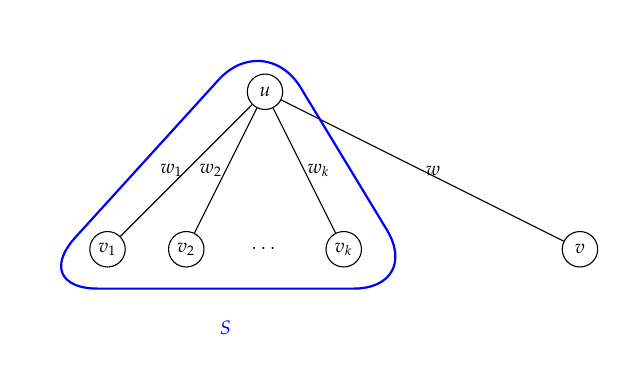
\begin{tikzpicture}[scale=1, every node/.style={inner sep=1pt}]
            \scriptsize
            % Nodes
            \node[draw, circle, minimum size=0.45cm] (u) at (-1, 2) {$u$};
            \node[draw, circle, minimum size=0.45cm] (v1) at (-3, 0) {$v_1$};
            \node[draw, circle, minimum size=0.45cm] (v2) at (-2, 0) {$v_2$};
            \node[draw, circle, minimum size=0.45cm] (vk) at (0, 0) {$v_k$};
            \node[draw, circle, minimum size=0.45cm] (v) at (3, 0) {$v$};

            % Connecting edges
            \draw (u) -- (v1) node[midway, left] {$w_1$};
            \draw (u) -- (v2) node[midway, left] {$w_2$};
            \draw (u) -- (vk) node[midway, right] {$w_k$};
            \draw (u) -- (v) node[midway, right] {$w$};

            % Dots
            \path (v2) -- (vk) node[midway, draw=none] {$\cdots$};

            % Enclosing large circle
           \draw[blue, thick, rounded corners=25pt] 
            (-4, -0.5) -- (1, -0.5) -- (-1, 2.8) -- cycle;
            \node[blue] at (-1.5, -1) {$S$};
        \end{tikzpicture}
    \end{minipage}
    \hfill
    \begin{minipage}{0.48\textwidth}
        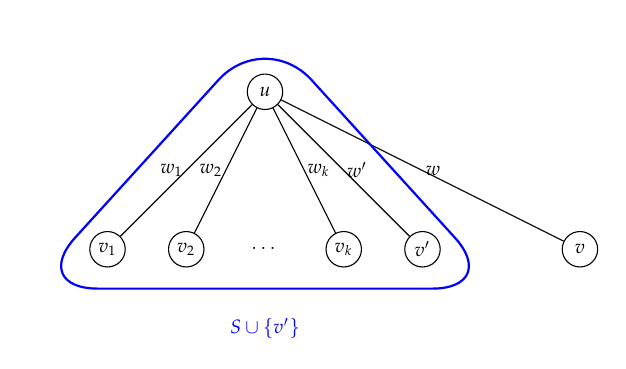
\begin{tikzpicture}[scale=1, every node/.style={inner sep=1pt}]
            \scriptsize
            % Nodes
            \node[draw, circle, minimum size=0.45cm] (u) at (-1, 2) {$u$};
            \node[draw, circle, minimum size=0.45cm] (v1) at (-3, 0) {$v_1$};
            \node[draw, circle, minimum size=0.45cm] (v2) at (-2, 0) {$v_2$};
            \node[draw, circle, minimum size=0.45cm] (vk) at (0, 0) {$v_k$};
            \node[draw, circle, minimum size=0.45cm] (v) at (3, 0) {$v$};
            \node[draw, circle, minimum size=0.45cm] (v') at (1, 0) {$v'$};

            % Connecting edges
            \draw (u) -- (v1) node[midway, left] {$w_1$};
            \draw (u) -- (v2) node[midway, left] {$w_2$};
            \draw (u) -- (vk) node[midway, right] {$w_k$};
            \draw (u) -- (v') node[midway, right] {$w'$};
            \draw (u) -- (v) node[midway, right] {$w$};

            % Dots
            \path (v2) -- (vk) node[midway, draw=none] {$\cdots$};

            % Enclosing large circle
           \draw[blue, thick, rounded corners=25pt] 
            (-4, -0.5) -- (2, -0.5) -- (-1, 2.8) -- cycle;
             \node[blue] at (-1, -1) {$S\cup\{v'\}$};
        \end{tikzpicture}
    \end{minipage}
    \caption{Graphs used in proof of \Cref{cl:marginal_utility}}
    \label{fig:marginal_utility}
\end{figure}


    Consider the graphs in the~\Cref{fig:marginal_utility}. Note that, for star graphs, a max. wt. $b$-matching can just be found by greedily picking the heaviest edges incident on $u$ up to a capacity of $b_{v_i}$ for each $v_i$. 
    
    Let the \textit{weights} of a max. wt. $b$-matching on $S$ be $e_1\geq e_2\geq \ldots \geq e_l$ and that on $S\cup \{v'\}$ be $f_1\geq f_2\geq \ldots \geq f_m$, where $m,l \leq b_u$. Since every edge available in $S$ is also available in $S\cup \{v'\}$, we have $l\leq m$. Let us extend the sequence $e_1\geq e_2\geq \ldots $ up to $m$ terms by adding zeros at the end. As the algorithm is greedy, we also have that $$\forall i\in \{1,2,\ldots,m\} , \quad e_i\leq f_i$$Now bring the vertex $v$ into the graph $S\cup \{v'\}$. Let it replace edges $f_{i_1} \geq f_{i_2} \geq \ldots \geq f_{i_t}$ with the edge $(u,v)$ of weight $w$ to get the max. wt. $b$-matching of $S\cup \{v,v'\}$. Then, replacing the corresponding edges $e_{i_1} \geq e_{i_2} \geq \ldots \geq  e_{i_t}$ with the edge $(u,v)$ will give us a valid $b$-matching in the graph $S\cup \{v\}$. And so, $$\nu(S\cup \{v,v'\}) - \nu(S\cup \{v'\}) = \sum_{j=i}^{t}(w-f_{i_j}) \leq \sum_{j=i}^{t}(w-e_{i_j}) \leq \nu(S\cup \{v\}) - \nu(S)$$ The first inequality comes from $e_i\leq f_i$ and the second inequality is true as the matching obtained by replacing edges $e_{i_1}, e_{i_2},\ldots, e_{i_t}$ with the edge $(u,v)$ need not be the max. wt. $b$-matching in $S\cup \{v\}$. This completes the claim. 
    
    
 \end{proof} 


\begin{corollary}
\label{cr:imputation_star}
There exists a polynomial time algorithm to decide if an imputation is in the core of $b$-matching games on star graphs.
\end{corollary}
%\todo{theorem 3 and 1 are similar ...}

\begin{proof}
    From~\Cref{lem:core_marginal_utility}, we only need to compute the marginal utilities of each leaf agent. And marginal utilities of each leaf agent $v_i$ can be computed just by solving for the max. wt. $b$-matching in $G$ and $G\setminus\{v_i\}$. \cite{Schrijver_book} details a strongly polynomial algorithm to compute the max. wt. $b$-matching in a graph. Combining the above, we get a strongly polynomial time algorithm to decide if an imputation is in the core of $b$-matching games on star graphs.
\end{proof}

\subsection{Unstable Coalitions under General Profit Shares}

\begin{definition}
    Given a cooperative game $G=(N,\nu)$ and a profit share $p$, an \textit{unstable coalition} $S\subseteq N$ is a set of agents who receive a profit less than their worth, i.e., $p(S)<\nu(S)$.
\end{definition}

Under this profit share, such sub-coalitions will break away from the grand coalition and hence cause instability. Given a profit share, our goal is to decide if such unstable sub-coalitions exist. The below theorem shows that the task is intractable.

\begin{theorem}
\label{thm:profit_share_for_star}
    Given a $b$-matching game on a star graph and a profit share, deciding if there exists an unstable sub-coalition is NP-complete.
    % \todo{Think about the definition of core for the profit share}
\end{theorem}

%\begin{theorem}
%    There is a pseudo-polynomial time algorithm to decide if a profit share is in the core of $b$-matching games on star graphs.
%\end{theorem}


\begin{proof}

%\todo[inline]{Replace all capital v and capital p to small letters. Ensure the notation is consistent with the notation and terms defined in the preliminaries.}

In this section, we will use the reduction from the \textsc{0-1 Knapsack Problem} which is stated as follows:
\begin{center}
\begin{tabular}{|>{\centering\arraybackslash}m{2cm}|m{10cm}|}
\hline
\multicolumn{2}{|c|}{\textsc{0-1 Knapsack Problem}} \\ \hline
\textbf{Instance:} & A set of $ n $ items $ \{1, 2, \dots, n\} $, each with a weight $ c_i \in \mathbb{N}$ and a value $ a_i \in \mathbb{N} $, and a knapsack with a maximum weight capacity $ C \in \mathbb{N} $ and a goal value $A \in \mathbb{N}$. \\ \hline
\textbf{Question:} & Is there a collection of items $ S \subseteq \{1, 2, \dots, n\} $ such that the total weight $ \sum_{i \in S} c_i \leq C $ and the total value $ \sum_{i \in S} a_i > A$ \\ \hline
\end{tabular}
\end{center}
Consider the following star graph $G^*$.
\begin{figure}[H]
    \centering
    \begin{tikzpicture}[scale=1.5, every node/.style={inner sep=1pt}]
        \small
        % Nodes
        \node[draw, circle, minimum size=0.45cm] (u) at (0, 2) {$u$};
        \node[draw, circle, minimum size=0.45cm] (v1) at (-3, 0) {$v_1$};
        \node[draw, circle, minimum size=0.45cm] (v2) at (-1, 0) {$v_2$};
        \node[draw, circle, minimum size=0.45cm] (vn) at (2.5, 0) {$v_n$};
        
        % Connecting edges
        \draw (u) -- (v1) node[midway, left] {$w_1$};
        \draw (u) -- (v2) node[midway, left] {$w_2$};
        \draw (u) -- (vn) node[midway, right] {$w_n$};
      
        % Dots
        \path (v2) -- (vn) node[midway, draw=none] {$\cdots$};
    \end{tikzpicture}
    \caption{Graph $G^*$ used in proof of~\Cref{thm:profit_share_for_star}}
    \label{fig:star}
\end{figure}
% \begin{center}
% \begin{tikzpicture}[scale=1.5, every node/.style={inner sep=1pt}]

% % Nodes
% \node[draw, circle, minimum size=0.6cm] (u) at (0, 2) {$u$};
% \node[draw, circle, minimum size=0.6cm] (v1) at (-2, 0) {$v_1$};
% \node[draw, circle, minimum size=0.6cm] (v2) at (-1, 0) {$v_2$};
% \node[draw, circle, minimum size=0.6cm] (vn) at (2, 0) {$v_n$};

% % Connecting edges
% \draw (u) -- (v1) node[midway, above left] {$w_1$};
% \draw (u) -- (v2) node[midway, above left] {$w_2$};
% \draw (u) -- (vn) node[midway, above right] {$w_n$};

% % Dots
% \path (v2) -- (vn) node[midway, draw=none] {$\cdots$};

% \end{tikzpicture}
% \end{center}


% we are going to prove that deciding if a profit share satisfies all core constraints even for star graphs is co-Np-hard. In this regard, we use a reduction from KNApSACK pROBLEM. 


%Let there be $ n $ items, where the $ i $-th item has value $ a_i $ and weight $ c_i $. The goal is to decide if a subset $ S $ of items satisfies:
%$
%\sum_{i \in S} c_i \leq C \quad \text{and} \quad \sum_{i \in S} a_i > A.
%$

Let $G^*=(U^*,V^*,E^*)$ such that $U^*= \{u\} , V^*=\{v_1,v_2, \ldots,$ $ v_n\}, E^*= \{(u,v_1),(u,v_2), \dots, (u,v_n)\}$. Represent $w: E^* \rightarrow \mathbb{R}_+$, $b: U^*\cup V^* \rightarrow \mathbb{Z}_+$ and $p: U^*\cup V^* \rightarrow \mathbb{R}_+$ as follows.

$$b_i:= b(v_i), \quad w_i:= w((u,v_i)) ,   \quad b_u:=b(u) , \quad p_i:= p(v_i), \quad p_u:=p(u)$$

Construct the instance based on knapsack instance as follows:
$
b_i = c_i, \quad w_i = a_i + 1, \quad p_i = -a_i + c_i(a_i + 1),\quad b_u= C, \quad p_u= A.
$
Let $S \subseteq U^*\cup V^*$ be a sub-coalition then: 
%and $v_i \in S$ be an agent that is not fully matched in a max. wt. $b$-matching in $S$. Then:
\begin{lemma}
\label{lem:fully_matched_in_star}
If $ v_i \in S $ and $ v_i $ is not fully matched in a max. wt.$ b $-matching in $ S $, then:
$
\nu(S) - p(S) < \nu(S \setminus \{v_i\}) - p(S \setminus \{v_i\}).
$

\end{lemma}

\begin{proof}
Removing $ v_i $ decreases $ p $ by $ p_i $, and as $v_i$ is not fully matched it decreases $ v $ by at most $ (b_i - 1)w_i $ Thus,
$
\nu(S) - p(S) \text{ increases by at least } p_i - (b_i - 1)w_i,
$
which simplifies to $ 1 $. Hence, $ \nu(S) - p(S)$ increases with the addition of $v_i$.

\end{proof}
\begin{corollary}
\label{cor:fully_matched}
    If $S\subseteq U^*\cup V^*$ is a sub-coalition that maximizes $\nu(S) - p(S)$ then every leaf player of $S$ must be fully matched in all max. wt. $b$-matching in $S$.
\end{corollary}
 
We want to check whether all sub-coalitions $S \subseteq U^*\cup V^*$ satisfy $\nu(S) - p(S) \leq 0$. This is true if the condition holds for all sub-coalitions $S$ that maximize the value of $\nu(S) - p(S)$. \Cref{cor:fully_matched} implies that such coalitions must fully match all their leaf players in their max. wt. $b$-matchings. So let us compute the values of $p(S)$ and $\nu(S)$ for these sets.

\begin{lemma}
    \label{lem:value_in_star}
    Assume that in a max. wt. $b$-matching on a sub-coalition of agents $S$, every vertex in $S \cap V^*$ is fully matched. Then the value of this subset is $\sum_{i \in S\cap v} a_i - A$. 
\end{lemma}
%\subsection{Computing the value}
%Assume that in a max. wt. $b$-matching on $S$ every vertices in $S \cap V$ are fully matched. The value of this subset is 
%$
%\nu(S)= \sum_{i \in S\cap v} b_iw_i
%$
%So:
%$
%\nu(S) - p(S) = (\sum_{i \in S\cap v} b_i w_i) - (\sum_{i \in S\cap v} p_i) - p_u.
%$

%Substituting the values:
%$
%\nu(S) - p(S) = \sum_{i \in S\cap v} c_i(a_i + 1) - \sum_{i \in S\cap v} (c_i(a_i + 1) - a_i) - A,
%$
%Which simplifies to:
%$
%\nu(S) - p(S) = \sum_{i \in S\cap v} a_i - A.
%$
\begin{proof}
All leaf vertices are fully matched so for each leaf vertex $v_i\in S$ it increases the value of $S$ by $b_iw_i$ so:
\begin{align*}
\nu(S) & = \sum_{i \in S \cap v} b_i w_i \\
\nu(S) - p(S) & = \sum_{i \in S \cap v} b_i w_i - \bigg(\sum_{i \in S \cap v} p_i + p_u \bigg) \\
 & = \sum_{i \in S \cap v} c_i (a_i + 1) - \bigg(\sum_{i \in S \cap v} (c_i (a_i + 1) - a_i) + A\bigg) \\
 & = \sum_{i \in S \cap v} a_i - A
\end{align*}
 \end{proof}
If there is a sub-coalition of agents $S$ such that $ \nu(S) - p(S) > 0 $, then we have a collection of items in \textsc{0-1 Knapsack Problem} such that the sum of their values is greater than $A$ and the sum of their weights does not exceed the capacity $C$ because the corresponding sub-coalition of this collection makes a valid $b$-matching, so it is satisfying the knapsack constraints. Conversely, any subset $ S' $ satisfying the knapsack constraints corresponds to an unstable coalition$ S $. So the reduction from \textsc{0-1 Knapsack Problem} is complete.
\end{proof}




    \section{General Bipartite Graphs}
\label{sec:general}
In this section, we will show how the NP-completeness result in star graphs results in NP-hardness of recognizing core imputations of general bipartite graphs. We will also show that this, in turn, translates to the NP-hardness of recognizing if an imputation is the leximin(or leximax) core imputation.  
% \todo {talk about leximin and leximax}

\subsection{Core imputations}

\begin{theorem}
\label{thm:core_coNP_complete}
    Deciding if an imputation is in the core of $b$-matching games on general bipartite graphs is co-NP-Complete.
\end{theorem}
% \todo {how can we handle the long proof of this theorem?}


% \begin{theorem}
%     There's a pseudo-polynomial time algorithm to check if a profit share is in the core of $b$-matching games on general bipartite graphs graphs.
% \end{theorem}

\begin{proof}
Clearly, the problem lies in co-NP, since a co-NP certificate for this problem would be a sub-coalition which is not satisfied under the imputation.\\ 
We will prove that deciding if an imputation is in the core of a bipartite $b$-matching game is co-NP-hard. In this regard, we use a reduction from the problem in~\Cref{thm:profit_share_for_star}. We will construct a bipartite graph $G'$ by adding 2 vertices to a star graph $G$ such that, there is an unstable sub-coalition of agents $S$ in $G'$ if and only if $S$ is an unstable coalition in $G$.

%We aim to transform the star graph of Lemma 1 into a graph $ G $ such that determining whether an imputation belongs to the core of $ G $ reduces to deciding whether a semi-imputation belongs to the semi-core of the original star graph. Specifically, we will add vertices $ x $ and $ y $ to the star graph, ensuring that any unstable coalitions of the resulting graph $ G $ correspond to unstable coalitions of the original star graph.

\begin{figure}[H]
    \centering
    \begin{minipage}{0.48\textwidth}
        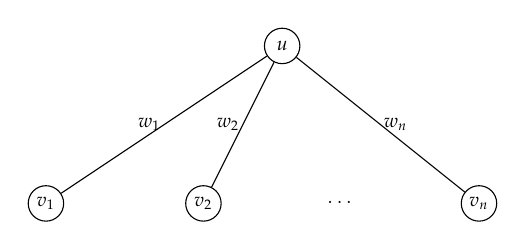
\begin{tikzpicture}[scale=1, every node/.style={inner sep=1pt}]
            \scriptsize
            % Nodes
            \node[draw, circle, minimum size=0.45cm] (u) at (0, 2) {$u$};
            \node[draw, circle, minimum size=0.45cm] (v1) at (-3, 0) {$v_1$};
            \node[draw, circle, minimum size=0.45cm] (v2) at (-1, 0) {$v_2$};
            \node[draw, circle, minimum size=0.45cm] (vn) at (2.5, 0) {$v_n$};

            % Connecting edges
            \draw (u) -- (v1) node[midway, left] {$w_1$};
            \draw (u) -- (v2) node[midway, left] {$w_2$};
            \draw (u) -- (vn) node[midway, right] {$w_n$};
            % Dots
            \path (v2) -- (vn) node[midway, draw=none] {$\cdots$};
        \end{tikzpicture}
    \end{minipage}
    \hfill
    \begin{minipage}{0.48\textwidth}
        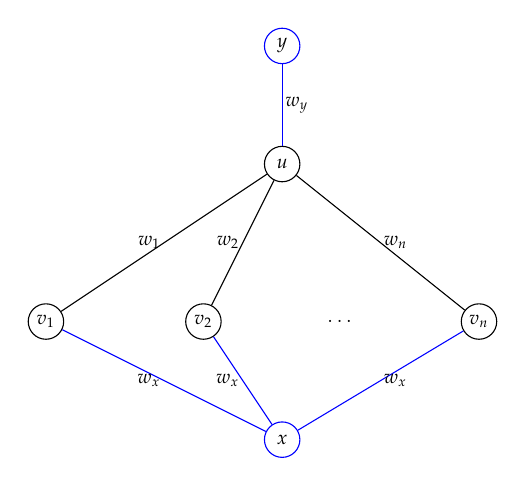
\begin{tikzpicture}[scale=1, every node/.style={inner sep=1pt}]
            \scriptsize
            % Nodes
            \node[draw, circle, minimum size=0.45cm] (u) at (0, 2) {$u$};
            \node[draw=blue, circle, minimum size=0.45cm] (y) at (0, 3.5) {$y$};
            \node[draw, circle, minimum size=0.45cm] (v1) at (-3, 0) {$v_1$};
            \node[draw, circle, minimum size=0.45cm] (v2) at (-1, 0) {$v_2$};
            \node[draw, circle, minimum size=0.45cm] (vn) at (2.5, 0) {$v_n$};
            \node[draw=blue, circle, minimum size=0.45cm] (x) at (0, -1.5) {$x$};

            % Connecting edges
            \draw (u) -- (v1) node[midway, left] {$w_1$};
            \draw (u) -- (v2) node[midway, left] {$w_2$};
            \draw (u) -- (vn) node[midway, right] {$w_n$};
            \draw[draw=blue] (u) -- (y) node[midway, right] {$w_y$};
            \draw[draw=blue] (v1) -- (x) node[midway, left] {$w_x$};
            \draw[draw=blue] (v2) -- (x) node[midway, left] {$w_x$};
            \draw[draw=blue] (vn) -- (x) node[midway, right] {$w_x$};

            % Dots
            \path (v2) -- (vn) node[midway, draw=none] {$\cdots$};
        \end{tikzpicture}
    \end{minipage}
    \caption{(Left) $G^*;\quad\quad$(Right) Add blue vertices and edges to $G^*$ to get $G$  }
    \label{fig:side_by_side_graph}
\end{figure}

%  \begin{center}
%     \begin{tikzpicture}[scale=1.5, every node/.style={inner sep=1pt}]
%         \small
%         % Nodes
%         \node[draw, circle, minimum size=0.45cm] (u) at (0, 2) {$u$};
%         \node[draw=blue, circle, minimum size=0.45cm] (y) at (0, 3.5) {$y$};
%         \node[draw, circle, minimum size=0.45cm] (v1) at (-3, 0) {$v_1$};
%         \node[draw, circle, minimum size=0.45cm] (v2) at (-1, 0) {$v_2$};
%         \node[draw, circle, minimum size=0.45cm] (vn) at (2.5, 0) {$v_n$};
%         \node[draw=blue, circle, minimum size=0.45cm] (x) at (0, -1.5) {$x$};

        
%         % Connecting edges
%         \draw (u) -- (v1) node[midway, left] {$w_1$};
%         \draw (u) -- (v2) node[midway, left] {$w_2$};
%         \draw (u) -- (vn) node[midway, right] {$w_n$};
%         \draw[draw=blue] (u) -- (y) node[midway, right] {$w_y$};
%         \draw[draw=blue] (v1) -- (x) node[midway, left] {$w_x$};
%         \draw[draw=blue] (v2) -- (x) node[midway, left] {$w_x$};
%         \draw[draw=blue] (vn) -- (x) node[midway, right] {$w_x$};

      
%         % Dots
%         \path (v2) -- (vn) node[midway, draw=none] {$\cdots$};
%     \end{tikzpicture}
% \end{center}
% \begin{center}
%     \begin{tikzpicture}[scale=1.5, every node/.style={inner sep=1pt}]

% % Nodes
% \node[draw, circle, minimum size=0.6cm] (u) at (0, 2) {$u$};
% \node[draw, circle, minimum size=0.6cm] (y) at (0, 3.5) {$y$};
% \node[draw, circle, minimum size=0.6cm] (v1) at (-2, 0) {$v_1$};
% \node[draw, circle, minimum size=0.6cm] (v2) at (-1, 0) {$v_2$};
% \node[draw, circle, minimum size=0.6cm] (vn) at (2, 0) {$v_n$};
% \node[draw, circle, minimum size=0.6cm] (x) at (0, -1.5) {$x$};

% % Connecting edges
% \draw (u) -- (v1) node[midway, left] {$w_1$};
% \draw (u) -- (v2) node[midway, left] {$w_2$};
% \draw (u) -- (vn) node[midway, right] {$w_n$};
% \draw (u) -- (y) node[midway, right] {$w_y$};
% %\draw[bend left] (y) to node[midway, above] {$w_y$} (u);
% \draw (v1) -- (x) node[midway, left] {$w_x$};
% \draw (v2) -- (x) node[midway, left] {$w_x$};
% \draw (vn) -- (x) node[midway, right] {$w_x$};

% % Dots
% \path (v2) -- (vn) node[midway, draw=none] {$\cdots$};

% \end{tikzpicture}
% \end{center}

To construct $ G=(U,V,E) $ consider same graph $G^*=(U^*,V^*,E^*)$ of~\Cref{thm:profit_share_for_star} and we add two vertices $x$ and $y$ as follows:
\begin{itemize}
    \item vertex $ x $ is connected to all $ v_i $ with edges of weight $ w_x $.
    \item vertex $ y $ is connected to $ u $ with an edge of weight $ w_y $.
\end{itemize}
%\todo{define $G'$ better}
So we have $G=(U,V,E)$ such that $U=U^* \cup\{x\}$, $V=V^*\cup\{y\}$, $E=E^*\cup\{(y,u),(x,v_1),$ $(x,v_2),\dots,(x,v_n)\}$

The parameters of the graph are defined as follows:
$$
w_x = \sum_{i=1}^n p_i + 1, \quad w_y = p_u + 1,
$$
$$
b_x = \sum_{i=1}^n b_i, \quad b_y = b_u,
$$
$$
p_x = (b_x - 1)w_x + 1, \quad p_y = (b_y - 1)w_y + 1.
$$


Firstly, we show that $p$ is an imputation in $G$, i.e., we need to show that $p(G) = \nu(G)$. So let us compute these values.

\begin{claim}
    $$p(G) = b_xw_x + b_yw_y$$
\end{claim}

\begin{proof}
The profit $ p(G) $ is the sum of profits assigned to all vertices:
    \begin{align*}
p(G) & = p_x + p_y + p_u + \sum_{i=1}^n p_i.\\
& = (b_x - 1)w_x + 1 + (b_y - 1)w_y + 1 + p_u + \sum_{i=1}^n p_i.\\
 &= b_x w_x - w_x + 1 + b_y w_y - w_y + 1 + p_u + \sum_{i=1}^n p_i\\
 &= b_x w_x - \left( \sum_{i=1}^n p_i + 1 \right) + 1 + b_y w_y - (p_u + 1) + 1 + p_u + \sum_{i=1}^n p_i.\\
\Rightarrow p(G) &= b_x w_x + b_y w_y.
\end{align*}
\end{proof}

% \subsection*{Computing $ p(G') $}
% \todo{Should we remove this part? I wrote it as a claim}
% The profit $ p(G') $ is the sum of profits assigned to all vertices:
% $
% p(G') = p_x + p_y + p_u + \sum_{i=1}^n p_i.
% $
% Substituting the definitions:
% $
% p(G') = (b_x - 1)w_x + 1 + (b_y - 1)w_y + 1 + p_u + \sum_{i=1}^n p_i.
% $
% Simplifying:
% $
% p(G') = b_x w_x - w_x + 1 + b_y w_y - w_y + 1 + p_u + \sum_{i=1}^n p_i.
% $
% Expanding $ w_x $ and $ w_y $:
% $
% p(G') = b_x w_x - \left( \sum_{i=1}^n p_i + 1 \right) + 1 + b_y w_y - (p_u + 1) + 1 + p_u + \sum_{i=1}^n p_i.
% $
% This simplifies to:
% $
% p(G') = b_x w_x + b_y w_y.
% $
\begin{claim}
    $$\nu(G') = b_xw_x+b_yw_y$$
\end{claim}
\begin{proof}
    The value $ \nu(G) $ is the max. wt. $ b $-matching in the graph $ G $. First, we show that in the max. wt. $ b $-matching of $ G $, no edge of the form $ (u,v_i) $ is used.
 
Suppose an edge $ (u,v_i) $ is included in the max. wt. $ b $-matching. We can remove this edge and instead add the edges $ (x,v_i) $ and $ (y,u) $. The value of the game then decreases by $ w_i $, from removing $ (u,v_i) $, but increases by $ w_x + w_y $, from adding $ (x,v_i) $ and $ (y,u) $). Since,
$$
w_x + w_y = \left( \sum_{i=1}^n p_i + 1 \right) + \left( p_u + 1 \right) = p(G) + 2,
$$
and $ p(G) + 2 > w_i $, this contradicts the maximality of the $ b $-matching.

Hence, no edges of the form $ (u,v_i) $ are used in the max. wt. $ b $-matching. Therefore, we can choose all edges adjacent to $x$ and $y$ upto their full capacities, without exceeding the capacities of other vertices to get the max. wt. $b$-matching. Hence, 
$
\nu(G') = b_x w_x + b_y w_y.
$
\end{proof}
\begin{corollary}
    $p(G) = \nu(G)$ so $p$ is an imputation for $G$.
\end{corollary}
% \subsection*{Computing $ \nu(G') $}
% \todo{Should we remove this part? I write it as a claim}
% The value $ \nu(G') $ is the max. wt. $ b $-matching in the graph $ G' $. First, we show that in the max. wt. $ b $-matching of $ G' $, no edge of the form $ uv_i $ is used.

% \textbf{proof by contradiction:}  
% Suppose an edge $ uv_i $ is included in the max. wt. $ b $-matching. We can remove this edge and instead add the edges $ xv_i $ and $ yu $. The value of the game then decreases by $ w_i $ (from removing $ uv_i $) but increases by $ w_x + w_y $ (from adding $ xv_i $ and $ yu $). Since:
% $
% w_x + w_y = \left( \sum_{i=1}^n p_i + 1 \right) + \left( p_u + 1 \right) = p(G') + 2,
% $
% and $ p(G') + 2 > w_i $, this contradicts the maximality of the $ b $-matching.

% Hence, no edges of the form $ uv_i $ are used in the max. wt. $ b $-matching. Therefore:
% $
% \nu(G') = b_x w_x + b_y w_y.
% $

% From the above, we conclude:
% $
% p(G') = \nu(G').
% $

%Now, we want to prove that if there is an unstable coalition such $S$ ($p(S) < \nu(S)$) then $S \cap \{x,y\} = \emptyset $. In this regard, we first prove a similar property as lemma \ref{fully matched in star}.

\begin{lemma}
    Let $S$ be an unstable coalition containing $x$ or $y$ which are not fully matched in any max. wt. $b$-matching in $S$. Then $S\setminus \{x,y\}$ is also an unstable coalition. 
  % Let $S \subseteq U\cup V$ such that $\nu(S) > p(S)$. If there exists a vertex $v \in \{x,y\}$ and $v\in S$ and $v$ is not fully matched in the max. wt. $b$-matching of $S$ then:
  % $$\nu(S \backslash\{v\}) > p(S\backslash\{v\})$$
\end{lemma}

\begin{proof}
Let us consider both cases. \\
\begin{itemize}
\vspace{-6mm}
    \item[] \textbf{Case(\textit{i}): }$v = x$ : 

        Removing $ x $ decreases the profit by $ p_x $ and as $x$ is not fully matched, the value is decreased by at most $ (b_x - 1)w_x $ Thus, $\nu(S) - p(S) \text{ increases by at least } p_x - (b_x - 1)w_x$.

    \item[]\textbf{Case(\textit{ii}): $v = y$} : 
        
        By a similar argument as above we can say that by removing $v_y$, $\nu(S) - p(S)$ increases by at least $ p_y - (b_y - 1)w_y$.
        
\end{itemize}
       
    As we have $p_x - (b_x - 1)w_x = p_y - (b_y - 1)w_y = 1 $, in both cases $\nu(S \backslash\{v\}) - p(S\backslash\{v\}) > \nu(S) - p(S)$. So if $S$ is an unstable coalition that does not fully match $x$ or $y$, then $S\setminus{\{x,y\}}$ is also an unstable coalition. 
\end{proof}

\begin{observation}
    If $S$ is a sub-coalition that maximizes $\nu(S) - p(S)$ and contains $x$ or $y$, then they must be fully matched in every max. wt. $b$-matching of $S$.
    % There is a subset of vertices $S$ which maximizes $\nu(S) - p(S)$ such that if $x$ or $y$ is in it they have to be fully matched in the max. wt. $b$-matching of $S$
\end{observation}
\begin{claim}
    No unstable coalition in $G$ contains $x$ or $y$.
    % If there is a unstable coalition such $S$ ($p(S) < \nu(S)$) then $S \cap \{x,y\} = \emptyset $.
\end{claim}
\begin{proof}

Consider a set $ S $ that maximizes $ \nu(S) - p(S) $. If both $ x $ and $ y $ are in $ S $, they must be fully matched, which implies that all vertices should be included in $ S $. Hence, $ S = G $, and we obtain $ \nu(S) - p(S) = 0 $.

Now, consider the case where $ y $ is in $ S $ but $ x $ is not. Since $ y $ must be fully matched, the edge $ (u,y) $ is chosen to satisfy the capacity of $ u $. Consequently, no edge $ (u,v_i) $ can be matched. Because $ x $ is not in $ S $, the presence of any $ v_i $ does not increase the value of $ S $, and thus these vertices can be removed to maximize $ \nu(S) - p(S) $. Removing all such vertices, we obtain $ S = \{y,u\} $. However, this is not an unstable coalition, as shown by the following computation:
$$p(S) = p_y + p_u = (b_y - 1)w_y + 1 + p_u = (b_u - 1)(p_u + 1) + p_u = b_up_u + b_u $$
$$\nu(S) = b_y.w_y = b_u(p_u+1) = b_up_u + b_u$$

Thus, we have $ p(S) = \nu(S) $.

Next, consider the case where $ x $ is in $ S $ but $ y $ is not. In this scenario, $ x $ must be fully matched, utilizing the entire capacity of the vertices $ v_i $. As a result, these vertices cannot be matched to $ u $, so removing $ u $ further increases $ \nu(S) - p(S) $. This leads to $ S = \{ x,v_1,v_2,\dots,v_n\} $.


$$p(S)= p_x+\sum_{i=1}^n p_i= (b_x - 1)w_x + 1 + \sum_{i=1}^n p_i = (\sum_{i=1}^nb_i - 1)(\sum_{i=1}^np_i + 1) + 1 + \sum_{i=1}^np_i = (\sum_{i=1}^nb_i)(\sum_{i=1}^np_i+1) $$
$$\nu(S)= b_xw_x = (\sum_{i=1}^nb_i)(\sum_{i=1}^np_i+1)  $$

Thus, we again obtain $ p(S) = \nu(S) $.
\end{proof}

We proved that if there is an unstable coalition in $G'$ it has to be an unstable coalition in $G$ so deciding whether imputation $p$ is in the core of $G'$ is equivalent to deciding whether the profit share $p$ is in the core of $G$ which we have proved shown is co-NP-hard. This completes the proof of \cref{thm:core_coNP_complete}.
\end{proof}







\subsection{Fair core imputations}
Using the NP-hardness result above, we will show that finding certain fair core imputations is NP-hard. We will look at finding imputations that maximize the minimum profit or minimize the maximum profit of agents in the $b$-matching game.

\begin{theorem}
    Finding a core imputation that maximizes the minimum profit-share of any vertex in a $b$-matching game is NP-hard. Similarly, it is NP-hard to find a core imputation that minimizes the maximum prove-share of any agent.
\end{theorem}

\begin{proof}
    Consider the game used in \Cref{thm:core_coNP_complete}. It gives a $b$-matching game on graph $G=(U, V, E), w: E\rightarrow \mathbb{R}_+, b:U\cup V\rightarrow \mathbb{Z}_+$ and an imputation $p$ such that, there exists an unstable coalition $S$, if and only if the corresponding items provide a valid knapsack solution.  

    To prove that finding a core imputation that maximizes the minimum profit in a $b$-matching game is NP-hard, we will construct a new graph, $G'$, and provide a new imputation, $p'$, based on $G$ and $p$ such that the $p'$ will give equal profits to all the agents and that $p'$ is in the core of the $G'$ if and only if $p$ is in the core of $G$. Since $p'$ gives equal profit to all agents, if it is in the core, it maximizes the minimum profit of all agents among core imputations. This will imply that recognizing if an imputation is maximizing the minimum profit in a $b$-matching game is co-NP-hard. And as the problem of recognition is co-NP-hard, computation of such a core imputation is NP-hard.
% \begin{center}
%     \begin{tikzpicture}[scale=1.5, every node/.style={inner sep=1pt}]

% % Nodes
% \node[draw, circle, minimum size=0.6cm] (u) at (0, 2) {$u$};
% \node[draw, circle, minimum size=0.6cm] (y) at (0, 3.5) {$y$};
% \node[draw, circle, minimum size=0.6cm] (v1) at (-4+1, 0) {$v_1$};
% \node[draw, circle, minimum size=0.6cm] (v2) at (-1, 0) {$v_2$};
% \node[draw, circle, minimum size=0.6cm] (vn) at (2.5, 0) {$v_n$};
% \node[draw, circle, minimum size=0.6cm] (x) at (0, -1.5) {$x$};

% \node[draw=red, circle, minimum size=0.6cm] (u') at (0-1, 2) {$u'$};
% \node[draw=red, circle, minimum size=0.6cm] (y') at (0-1, 3.5) {$y'$};
% \node[draw=red, circle, minimum size=0.6cm] (v'1) at (-5+1, 0) {$v'_1$};
% \node[draw=red, circle, minimum size=0.6cm] (v'2) at (-1-1, 0) {$v'_2$};
% \node[draw=red, circle, minimum size=0.6cm] (v'n) at (1.5, 0) {$v'_n$};
% \node[draw=red, circle, minimum size=0.6cm] (x') at (0-1, -1.5) {$x'$};

% % Connecting edges
% \draw (u) -- (v1) node[midway, left] {$w_1$};
% \draw (u) -- (v2) node[midway, left] {$w_2$};
% \draw (u) -- (vn) node[midway, right] {$w_n$};
% \draw (u) -- (y) node[midway, right] {$w_y$};
% %\draw[bend left] (y) to node[midway, above] {$w_y$} (u);
% \draw (v1) -- (x) node[midway, left] {$w_x$};
% \draw (v2) -- (x) node[midway, left] {$w_x$};
% \draw (vn) -- (x) node[midway, right] {$w_x$};

% \draw[draw=red] (y) -- (y') node[midway, above] {$w'_y$};
% \draw[draw=red] (u) -- (u') node[midway, above] {$w'_u$};
% \draw[draw=red] (v1) -- (v'1) node[midway, above] {$w'_{v_1}$};
% \draw[draw=red] (v2) -- (v'2) node[midway, above] {$w'_{v_2}$};
% \draw[draw=red] (vn) -- (v'n) node[midway, above] {$w'_{v_n}$};
% \draw[draw=red] (x) -- (x') node[midway, above] {$w'_x$};

% % Dots
% \path (v2) -- (vn) node[midway, draw=none] {$\cdots$};

% \end{tikzpicture}
% \end{center}

% \begin{center}
%     \begin{tikzpicture}[scale=1.5, every node/.style={inner sep=1pt}]

% % Nodes
% \node[draw, circle, minimum size=0.6cm] (u) at (0, 2) {$u$};
% \node[draw, circle, minimum size=0.6cm] (y) at (0, 3.5) {$y$};
% \node[draw, circle, minimum size=0.6cm] (v1) at (-4+1, 0) {$v_1$};
% \node[draw, circle, minimum size=0.6cm] (v2) at (-1, 0) {$v_2$};
% \node[draw, circle, minimum size=0.6cm] (vn) at (2.5, 0) {$v_n$};
% \node[draw, circle, minimum size=0.6cm] (x) at (0, -1.5) {$x$};


% % Connecting edges
% \draw (u) -- (v1) node[midway, left] {$w_1$};
% \draw (u) -- (v2) node[midway, left] {$w_2$};
% \draw (u) -- (vn) node[midway, right] {$w_n$};
% \draw (u) -- (y) node[midway, right] {$w_y$};
% %\draw[bend left] (y) to node[midway, above] {$w_y$} (u);
% \draw (v1) -- (x) node[midway, left] {$w_x$};
% \draw (v2) -- (x) node[midway, left] {$w_x$};
% \draw (vn) -- (x) node[midway, right] {$w_x$};

% % Dots
% \path (v2) -- (vn) node[midway, draw=none] {$\cdots$};

% \end{tikzpicture}
% \end{center}
\begin{figure}[H]
    \centering
    \begin{minipage}{0.48\textwidth}
        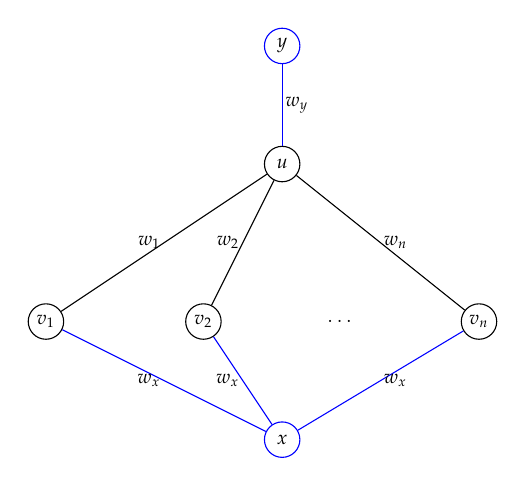
\begin{tikzpicture}[scale=1, every node/.style={inner sep=1pt}]
            \scriptsize
            % Nodes
            \node[draw, circle, minimum size=0.45cm] (u) at (0, 2) {$u$};
            \node[draw=blue, circle, minimum size=0.45cm] (y) at (0, 3.5) {$y$};
            \node[draw, circle, minimum size=0.45cm] (v1) at (-3, 0) {$v_1$};
            \node[draw, circle, minimum size=0.45cm] (v2) at (-1, 0) {$v_2$};
            \node[draw, circle, minimum size=0.45cm] (vn) at (2.5, 0) {$v_n$};
            \node[draw=blue, circle, minimum size=0.45cm] (x) at (0, -1.5) {$x$};

            % Connecting edges
            \draw (u) -- (v1) node[midway, left] {$w_1$};
            \draw (u) -- (v2) node[midway, left] {$w_2$};
            \draw (u) -- (vn) node[midway, right] {$w_n$};
            \draw[draw=blue] (u) -- (y) node[midway, right] {$w_y$};
            \draw[draw=blue] (v1) -- (x) node[midway, left] {$w_x$};
            \draw[draw=blue] (v2) -- (x) node[midway, left] {$w_x$};
            \draw[draw=blue] (vn) -- (x) node[midway, right] {$w_x$};

            % Dots
            \path (v2) -- (vn) node[midway, draw=none] {$\cdots$};
        \end{tikzpicture}
    \end{minipage}
    \hfill
    \begin{minipage}{0.48\textwidth}
        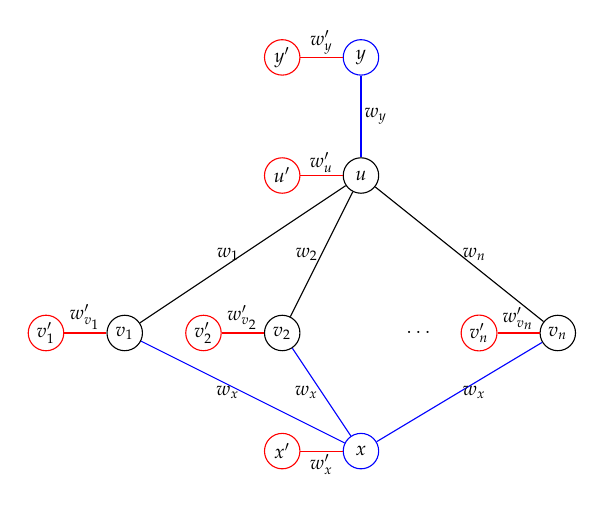
\begin{tikzpicture}[scale=1, every node/.style={inner sep=1pt}]
            \scriptsize
            % Nodes
            \node[draw, circle, minimum size=0.45cm] (u) at (0, 2) {$u$};
            \node[draw=blue, circle, minimum size=0.45cm] (y) at (0, 3.5) {$y$};
            \node[draw, circle, minimum size=0.45cm] (v1) at (-3, 0) {$v_1$};
            \node[draw, circle, minimum size=0.45cm] (v2) at (-1, 0) {$v_2$};
            \node[draw, circle, minimum size=0.45cm] (vn) at (2.5, 0) {$v_n$};
            \node[draw=blue, circle, minimum size=0.45cm] (x) at (0, -1.5) {$x$};

            \node[draw=red, circle, minimum size=0.45cm] (u') at (-1, 2) {$u'$};
            \node[draw=red, circle, minimum size=0.45cm] (y') at (-1, 3.5) {$y'$};
            \node[draw=red, circle, minimum size=0.45cm] (v'1) at (-4, 0) {$v'_1$};
            \node[draw=red, circle, minimum size=0.45cm] (v'2) at (-2, 0) {$v'_2$};
            \node[draw=red, circle, minimum size=0.45cm] (v'n) at (1.5, 0) {$v'_n$};
            \node[draw=red, circle, minimum size=0.45cm] (x') at (-1, -1.5) {$x'$};

            % Connecting edges
            \draw (u) -- (v1) node[midway, left] {$w_1$};
            \draw (u) -- (v2) node[midway, left] {$w_2$};
            \draw (u) -- (vn) node[midway, right] {$w_n$};
            \draw[draw=blue] (u) -- (y) node[midway, right] {$w_y$};
            \draw[draw=blue] (v1) -- (x) node[midway, left] {$w_x$};
            \draw[draw=blue] (v2) -- (x) node[midway, left] {$w_x$};
            \draw[draw=blue] (vn) -- (x) node[midway, right] {$w_x$};

            \draw[draw=red] (y) -- (y') node[midway, above] {$w'_y$};
            \draw[draw=red] (u) -- (u') node[midway, above] {$w'_u$};
            \draw[draw=red] (v1) -- (v'1) node[midway, above] {$w'_{v_1}$};
            \draw[draw=red] (v2) -- (v'2) node[midway, above] {$w'_{v_2}$};
            \draw[draw=red] (vn) -- (v'n) node[midway, above] {$w'_{v_n}$};
            \draw[draw=red] (x) -- (x') node[midway, below] {$w'_x$};

            % Dots
            \path (v2) -- (vn) node[midway, draw=none] {$\cdots$};
        \end{tikzpicture}
    \end{minipage}
    \caption{(Left) $G;\quad$(Right) We add partner vertices, shown in red, for every vertex in $G$ to get $G'$}
    \label{fig:extended_graph}
\end{figure}

    % \textbf{Construction:} \\
    % \todo[inline]{RG: Change $V$ to $U\cup V$.}
    We will construct $\{G',w',b'\}$ from $\{G,w,b\}$. Let $\nu$ and $\nu'$ represent the characteristic functions of the $b$-matching games in $G$ and $G'$ respectively.
    Construct the graph $G'=(U', V', E')$ from $G=(U, V, E)$ as follows. For every vertex $v$ in $U\cup V$, there are two vertices - $v, v'$ - in $U'\cup V'$. Call $v$'s as the \textit{original} vertices and $v'$'s, the \textit{partner} vertices of respective original vertex $v$.
    
    Preserve all the edges from $G$ in $G'$, i.e., if $(u,v)\in E$, then $(u,v)\in E'$. Weights of all such edges will remain the same. Add an edge between every vertex and its partner, i.e., $\forall v\in U\cup V, (v,v')\in E'$. The weights of these edges will be set based on the profits of agents in $p$ and weights of edges in $E$ as follows. Let $$p^* = 1+ \max{\{\max_{v\in U\cup V} p_v, \max_{e \in E} w_e \}}$$Then $$\forall v \in U\cup V,\quad w'_{(v,v')} = 2p^* - p_v$$ The capacities, $b':U'\cup V'\rightarrow \mathbb{Z}_+$ of all original vertices will be set one more than their capacities in $G$ and the capacities of partner vertices will be set to 1, i.e., $b'_v = 1 + b_v$ and $b'_{v'} = 1$.

    Note that $p^*$ is chosen so that for every vertex, the edge to its partner is heavier than all other edges incident on it - $$ w'_{(v,v')} = 2p^* - p_v = (p^* - p_v) + (p^*) > p^* > w_e,\forall {e \in E}$$ And since we have increased the capacities of all original vertices by 1 and set the capacities of all partner vertices to 1, this, in effect, ensures the following.

    \begin{claim}
    \label{cl:max_wt_b_matching}
        The max. wt. $b$-matching of $G'$ is some max. wt. $b$-matching in $G$ together with all edges between original vertices and their partners. 
    \end{claim}

    \begin{proof}
        Given any $b$-matching, not containing $(v,v')$ for some $v\in U\cup V$, we can include $(v,v')$, replacing any other edge incident on $v$ if necessary, to get another $b$-matching with a larger weight. Hence, every edge between an original vertex and its partner is chosen exactly once in the max. wt. $b$-matching in $G'$. Given these edges are chosen, the capacities on original vertices will become the same as in $G$, completing the proof.  
    \end{proof}

    Finally, consider the profit share $$\forall v\in U'\cup V', \quad p'(v) = p^*$$
    \begin{lemma}
        $p':U'\cup V'\rightarrow \mathbb{R}_+$ is an imputation in the $b$-matching game on $G'$.
    \end{lemma}

    \begin{proof}
        The total profit distributed by $p' = \sum_{v\in U'\cup V'} p^* = 2|(U'\cup V')|\cdot p^*$
        From \Cref{cl:max_wt_b_matching}, the total worth of the game is $\nu(G') = \nu(G)+\sum_{v\in U\cup V}(2p^*-p_v) = \nu(G) + 2|(U\cup V)|\cdot p^* - \sum_{v\in U\cup V} p_v$. Since $p:U\cup V\rightarrow \mathbb{R}_+$ is an imputation in $G$, $\sum_{v\in U\cup V} p_v = p(G) = \nu(G)$, and $\nu(G') = 2|U\cup V|\cdot p^* = p'(G')$. Hence, $p'$ is an imputation in the $b$-matching game on $G'$.
    \end{proof}

    Now we prove the main lemma. 

    \begin{lemma}
    \label{lem:leximin_reduction}
        $p'$ is not in the core of $(G',\nu')$ if and only if $p$ is not in the core of $(G,\nu)$.
    \end{lemma}

    \begin{proof}
        Assume $p$ is not in the core of $(G,\nu)$ as $p(S)<\nu(S)$ for some set $S\subseteq U\cup V$. Let $S'$ be the union of all original vertices and their partner vertices of every vertex in $S$. Then, like in the proof of \Cref{cl:max_wt_b_matching}, $$\nu'(S') = \nu(S) + \sum_{v\in S}(2p^*-p_v) = \nu(S) + 2|S|\cdot p^* - \sum_{v\in S}(p_v) = \nu(S) + 2|S|\cdot p^* - p(S)$$Also note that $p'(S') = 2|S|\cdot p^*$ as every vertex $v$ in $S'$ gets the same profit of $p^*$. Therefore $p(S) < \nu(S) \implies p'(S') < \nu'(S')$. This shows that if $p$ is not in the core of $(G,\nu)$ then $p'$ is not in the core of $(G',\nu')$.
        
    

        Now assume $p'$ is not in the core of $(G',\nu')$. Let $S^*\subseteq U'\cup V'$ be a \textit{minimal} set such that $p'(S^*)<\nu'(S^*)$. Note that, for every partner vertex $v'\in S^*$, $S^*$ must also contain the original vertex $v$. For otherwise, we can remove $v'$ from $S^*$ decreasing the profit but not the worth, contradicting the minimality of $S^*$.        
        
        Now, if $S^*$ contains an original vertex $v$ but not its partner $v'$, we can add $v'$ to $S^*$ and still maintain $p'(S^*\cup \{v'\})<\nu'(S^* \cup \{v'\})$ as this increases the value($2p^*-p_v$) more than the profit($p^*$). performing this operation for all original vertices, we will end up with a set $S'$ which has a vertex and its partners in pairs, and $p'(S') < \nu'(S')$.

        Now consider the sub-coalition of agents $S$ of just the original partner vertices in $S'$, in the game $(G,\nu)$. Note that, like above, $p'(S') = 2|S|\cdot p^*$ and $\nu'(S') = \nu(S) + \sum_{v\in S}(2p^*-p_v) = \nu(S) + 2|S|\cdot p^* - \sum_{v\in S}(p_v) = \nu(S) + 2|S|\cdot p^* - p(S)$.

        And so, if $p'(S') < \nu'(S')$ then $p(S) < \nu(S)$ proving the other direction of the lemma.
        
    \end{proof}

    Combining \Cref{lem:leximin_reduction} and \Cref{thm:core_coNP_complete}, we get that finding an unstable coalition in $(G',\nu')$ under imputation $p'$ is NP-hard. Since $p'$ is the imputation that distributes equal profit to all the agents, this proves that it is NP-hard to compute an imputation that maximizes the minimum profit or minimizes the maximum profit. 

\end{proof}

Since leximin and leximax imputations also maximize the minimum profit and minimize the maximum profit, it is also NP-hard to  compute them.

\begin{corollary}
\label{cor:leximin_NP_hard}
    Computing the leximin(or leximax) core imputation in a $b$-matching game is NP-hard.
\end{corollary}    

% \begin{theorem}
%     There's a pseudo-polynomial time algorithm to check if a profit share is in the core of $b$-matching games on general bipartite graphs graphs, with a constant number of vertices in one of the partitions.
% \end{theorem}


    
    \section{Discussion of Assumptions}\label{sec:discussion}
In this paper, we have made several assumptions for the sake of clarity and simplicity. In this section, we discuss the rationale behind these assumptions, the extent to which these assumptions hold in practice, and the consequences for our protocol when these assumptions hold.

\subsection{Assumptions on the Demand}

There are two simplifying assumptions we make about the demand. First, we assume the demand at any time is relatively small compared to the channel capacities. Second, we take the demand to be constant over time. We elaborate upon both these points below.

\paragraph{Small demands} The assumption that demands are small relative to channel capacities is made precise in \eqref{eq:large_capacity_assumption}. This assumption simplifies two major aspects of our protocol. First, it largely removes congestion from consideration. In \eqref{eq:primal_problem}, there is no constraint ensuring that total flow in both directions stays below capacity--this is always met. Consequently, there is no Lagrange multiplier for congestion and no congestion pricing; only imbalance penalties apply. In contrast, protocols in \cite{sivaraman2020high, varma2021throughput, wang2024fence} include congestion fees due to explicit congestion constraints. Second, the bound \eqref{eq:large_capacity_assumption} ensures that as long as channels remain balanced, the network can always meet demand, no matter how the demand is routed. Since channels can rebalance when necessary, they never drop transactions. This allows prices and flows to adjust as per the equations in \eqref{eq:algorithm}, which makes it easier to prove the protocol's convergence guarantees. This also preserves the key property that a channel's price remains proportional to net money flow through it.

In practice, payment channel networks are used most often for micro-payments, for which on-chain transactions are prohibitively expensive; large transactions typically take place directly on the blockchain. For example, according to \cite{river2023lightning}, the average channel capacity is roughly $0.1$ BTC ($5,000$ BTC distributed over $50,000$ channels), while the average transaction amount is less than $0.0004$ BTC ($44.7k$ satoshis). Thus, the small demand assumption is not too unrealistic. Additionally, the occasional large transaction can be treated as a sequence of smaller transactions by breaking it into packets and executing each packet serially (as done by \cite{sivaraman2020high}).
Lastly, a good path discovery process that favors large capacity channels over small capacity ones can help ensure that the bound in \eqref{eq:large_capacity_assumption} holds.

\paragraph{Constant demands} 
In this work, we assume that any transacting pair of nodes have a steady transaction demand between them (see Section \ref{sec:transaction_requests}). Making this assumption is necessary to obtain the kind of guarantees that we have presented in this paper. Unless the demand is steady, it is unreasonable to expect that the flows converge to a steady value. Weaker assumptions on the demand lead to weaker guarantees. For example, with the more general setting of stochastic, but i.i.d. demand between any two nodes, \cite{varma2021throughput} shows that the channel queue lengths are bounded in expectation. If the demand can be arbitrary, then it is very hard to get any meaningful performance guarantees; \cite{wang2024fence} shows that even for a single bidirectional channel, the competitive ratio is infinite. Indeed, because a PCN is a decentralized system and decisions must be made based on local information alone, it is difficult for the network to find the optimal detailed balance flow at every time step with a time-varying demand.  With a steady demand, the network can discover the optimal flows in a reasonably short time, as our work shows.

We view the constant demand assumption as an approximation for a more general demand process that could be piece-wise constant, stochastic, or both (see simulations in Figure \ref{fig:five_nodes_variable_demand}).
We believe it should be possible to merge ideas from our work and \cite{varma2021throughput} to provide guarantees in a setting with random demands with arbitrary means. We leave this for future work. In addition, our work suggests that a reasonable method of handling stochastic demands is to queue the transaction requests \textit{at the source node} itself. This queuing action should be viewed in conjunction with flow-control. Indeed, a temporarily high unidirectional demand would raise prices for the sender, incentivizing the sender to stop sending the transactions. If the sender queues the transactions, they can send them later when prices drop. This form of queuing does not require any overhaul of the basic PCN infrastructure and is therefore simpler to implement than per-channel queues as suggested by \cite{sivaraman2020high} and \cite{varma2021throughput}.

\subsection{The Incentive of Channels}
The actions of the channels as prescribed by the DEBT control protocol can be summarized as follows. Channels adjust their prices in proportion to the net flow through them. They rebalance themselves whenever necessary and execute any transaction request that has been made of them. We discuss both these aspects below.

\paragraph{On Prices}
In this work, the exclusive role of channel prices is to ensure that the flows through each channel remains balanced. In practice, it would be important to include other components in a channel's price/fee as well: a congestion price  and an incentive price. The congestion price, as suggested by \cite{varma2021throughput}, would depend on the total flow of transactions through the channel, and would incentivize nodes to balance the load over different paths. The incentive price, which is commonly used in practice \cite{river2023lightning}, is necessary to provide channels with an incentive to serve as an intermediary for different channels. In practice, we expect both these components to be smaller than the imbalance price. Consequently, we expect the behavior of our protocol to be similar to our theoretical results even with these additional prices.

A key aspect of our protocol is that channel fees are allowed to be negative. Although the original Lightning network whitepaper \cite{poon2016bitcoin} suggests that negative channel prices may be a good solution to promote rebalancing, the idea of negative prices in not very popular in the literature. To our knowledge, the only prior work with this feature is \cite{varma2021throughput}. Indeed, in papers such as \cite{van2021merchant} and \cite{wang2024fence}, the price function is explicitly modified such that the channel price is never negative. The results of our paper show the benefits of negative prices. For one, in steady state, equal flows in both directions ensure that a channel doesn't loose any money (the other price components mentioned above ensure that the channel will only gain money). More importantly, negative prices are important to ensure that the protocol selectively stifles acyclic flows while allowing circulations to flow. Indeed, in the example of Section \ref{sec:flow_control_example}, the flows between nodes $A$ and $C$ are left on only because the large positive price over one channel is canceled by the corresponding negative price over the other channel, leading to a net zero price.

Lastly, observe that in the DEBT control protocol, the price charged by a channel does not depend on its capacity. This is a natural consequence of the price being the Lagrange multiplier for the net-zero flow constraint, which also does not depend on the channel capacity. In contrast, in many other works, the imbalance price is normalized by the channel capacity \cite{ren2018optimal, lin2020funds, wang2024fence}; this is shown to work well in practice. The rationale for such a price structure is explained well in \cite{wang2024fence}, where this fee is derived with the aim of always maintaining some balance (liquidity) at each end of every channel. This is a reasonable aim if a channel is to never rebalance itself; the experiments of the aforementioned papers are conducted in such a regime. In this work, however, we allow the channels to rebalance themselves a few times in order to settle on a detailed balance flow. This is because our focus is on the long-term steady state performance of the protocol. This difference in perspective also shows up in how the price depends on the channel imbalance. \cite{lin2020funds} and \cite{wang2024fence} advocate for strictly convex prices whereas this work and \cite{varma2021throughput} propose linear prices.

\paragraph{On Rebalancing} 
Recall that the DEBT control protocol ensures that the flows in the network converge to a detailed balance flow, which can be sustained perpetually without any rebalancing. However, during the transient phase (before convergence), channels may have to perform on-chain rebalancing a few times. Since rebalancing is an expensive operation, it is worthwhile discussing methods by which channels can reduce the extent of rebalancing. One option for the channels to reduce the extent of rebalancing is to increase their capacity; however, this comes at the cost of locking in more capital. Each channel can decide for itself the optimum amount of capital to lock in. Another option, which we discuss in Section \ref{sec:five_node}, is for channels to increase the rate $\gamma$ at which they adjust prices. 

Ultimately, whether or not it is beneficial for a channel to rebalance depends on the time-horizon under consideration. Our protocol is based on the assumption that the demand remains steady for a long period of time. If this is indeed the case, it would be worthwhile for a channel to rebalance itself as it can make up this cost through the incentive fees gained from the flow of transactions through it in steady state. If a channel chooses not to rebalance itself, however, there is a risk of being trapped in a deadlock, which is suboptimal for not only the nodes but also the channel.

\section{Conclusion}
This work presents DEBT control: a protocol for payment channel networks that uses source routing and flow control based on channel prices. The protocol is derived by posing a network utility maximization problem and analyzing its dual minimization. It is shown that under steady demands, the protocol guides the network to an optimal, sustainable point. Simulations show its robustness to demand variations. The work demonstrates that simple protocols with strong theoretical guarantees are possible for PCNs and we hope it inspires further theoretical research in this direction.
    
    %% \smallskip
% \myparagraph{Acknowledgments} We thank the reviewers for their comments.
% The work by Moshe Tennenholtz was supported by funding from the
% European Research Council (ERC) under the European Union's Horizon
% 2020 research and innovation programme (grant agreement 740435).

    
    \bibliographystyle{alpha}
    % \bibliographystyle{abbrvnat}
    % \bibliographystyle{abbrv}
    \bibliography{refs}
    
    % \appendix
    % \subsection{Lloyd-Max Algorithm}
\label{subsec:Lloyd-Max}
For a given quantization bitwidth $B$ and an operand $\bm{X}$, the Lloyd-Max algorithm finds $2^B$ quantization levels $\{\hat{x}_i\}_{i=1}^{2^B}$ such that quantizing $\bm{X}$ by rounding each scalar in $\bm{X}$ to the nearest quantization level minimizes the quantization MSE. 

The algorithm starts with an initial guess of quantization levels and then iteratively computes quantization thresholds $\{\tau_i\}_{i=1}^{2^B-1}$ and updates quantization levels $\{\hat{x}_i\}_{i=1}^{2^B}$. Specifically, at iteration $n$, thresholds are set to the midpoints of the previous iteration's levels:
\begin{align*}
    \tau_i^{(n)}=\frac{\hat{x}_i^{(n-1)}+\hat{x}_{i+1}^{(n-1)}}2 \text{ for } i=1\ldots 2^B-1
\end{align*}
Subsequently, the quantization levels are re-computed as conditional means of the data regions defined by the new thresholds:
\begin{align*}
    \hat{x}_i^{(n)}=\mathbb{E}\left[ \bm{X} \big| \bm{X}\in [\tau_{i-1}^{(n)},\tau_i^{(n)}] \right] \text{ for } i=1\ldots 2^B
\end{align*}
where to satisfy boundary conditions we have $\tau_0=-\infty$ and $\tau_{2^B}=\infty$. The algorithm iterates the above steps until convergence.

Figure \ref{fig:lm_quant} compares the quantization levels of a $7$-bit floating point (E3M3) quantizer (left) to a $7$-bit Lloyd-Max quantizer (right) when quantizing a layer of weights from the GPT3-126M model at a per-tensor granularity. As shown, the Lloyd-Max quantizer achieves substantially lower quantization MSE. Further, Table \ref{tab:FP7_vs_LM7} shows the superior perplexity achieved by Lloyd-Max quantizers for bitwidths of $7$, $6$ and $5$. The difference between the quantizers is clear at 5 bits, where per-tensor FP quantization incurs a drastic and unacceptable increase in perplexity, while Lloyd-Max quantization incurs a much smaller increase. Nevertheless, we note that even the optimal Lloyd-Max quantizer incurs a notable ($\sim 1.5$) increase in perplexity due to the coarse granularity of quantization. 

\begin{figure}[h]
  \centering
  \includegraphics[width=0.7\linewidth]{sections/figures/LM7_FP7.pdf}
  \caption{\small Quantization levels and the corresponding quantization MSE of Floating Point (left) vs Lloyd-Max (right) Quantizers for a layer of weights in the GPT3-126M model.}
  \label{fig:lm_quant}
\end{figure}

\begin{table}[h]\scriptsize
\begin{center}
\caption{\label{tab:FP7_vs_LM7} \small Comparing perplexity (lower is better) achieved by floating point quantizers and Lloyd-Max quantizers on a GPT3-126M model for the Wikitext-103 dataset.}
\begin{tabular}{c|cc|c}
\hline
 \multirow{2}{*}{\textbf{Bitwidth}} & \multicolumn{2}{|c|}{\textbf{Floating-Point Quantizer}} & \textbf{Lloyd-Max Quantizer} \\
 & Best Format & Wikitext-103 Perplexity & Wikitext-103 Perplexity \\
\hline
7 & E3M3 & 18.32 & 18.27 \\
6 & E3M2 & 19.07 & 18.51 \\
5 & E4M0 & 43.89 & 19.71 \\
\hline
\end{tabular}
\end{center}
\end{table}

\subsection{Proof of Local Optimality of LO-BCQ}
\label{subsec:lobcq_opt_proof}
For a given block $\bm{b}_j$, the quantization MSE during LO-BCQ can be empirically evaluated as $\frac{1}{L_b}\lVert \bm{b}_j- \bm{\hat{b}}_j\rVert^2_2$ where $\bm{\hat{b}}_j$ is computed from equation (\ref{eq:clustered_quantization_definition}) as $C_{f(\bm{b}_j)}(\bm{b}_j)$. Further, for a given block cluster $\mathcal{B}_i$, we compute the quantization MSE as $\frac{1}{|\mathcal{B}_{i}|}\sum_{\bm{b} \in \mathcal{B}_{i}} \frac{1}{L_b}\lVert \bm{b}- C_i^{(n)}(\bm{b})\rVert^2_2$. Therefore, at the end of iteration $n$, we evaluate the overall quantization MSE $J^{(n)}$ for a given operand $\bm{X}$ composed of $N_c$ block clusters as:
\begin{align*}
    \label{eq:mse_iter_n}
    J^{(n)} = \frac{1}{N_c} \sum_{i=1}^{N_c} \frac{1}{|\mathcal{B}_{i}^{(n)}|}\sum_{\bm{v} \in \mathcal{B}_{i}^{(n)}} \frac{1}{L_b}\lVert \bm{b}- B_i^{(n)}(\bm{b})\rVert^2_2
\end{align*}

At the end of iteration $n$, the codebooks are updated from $\mathcal{C}^{(n-1)}$ to $\mathcal{C}^{(n)}$. However, the mapping of a given vector $\bm{b}_j$ to quantizers $\mathcal{C}^{(n)}$ remains as  $f^{(n)}(\bm{b}_j)$. At the next iteration, during the vector clustering step, $f^{(n+1)}(\bm{b}_j)$ finds new mapping of $\bm{b}_j$ to updated codebooks $\mathcal{C}^{(n)}$ such that the quantization MSE over the candidate codebooks is minimized. Therefore, we obtain the following result for $\bm{b}_j$:
\begin{align*}
\frac{1}{L_b}\lVert \bm{b}_j - C_{f^{(n+1)}(\bm{b}_j)}^{(n)}(\bm{b}_j)\rVert^2_2 \le \frac{1}{L_b}\lVert \bm{b}_j - C_{f^{(n)}(\bm{b}_j)}^{(n)}(\bm{b}_j)\rVert^2_2
\end{align*}

That is, quantizing $\bm{b}_j$ at the end of the block clustering step of iteration $n+1$ results in lower quantization MSE compared to quantizing at the end of iteration $n$. Since this is true for all $\bm{b} \in \bm{X}$, we assert the following:
\begin{equation}
\begin{split}
\label{eq:mse_ineq_1}
    \tilde{J}^{(n+1)} &= \frac{1}{N_c} \sum_{i=1}^{N_c} \frac{1}{|\mathcal{B}_{i}^{(n+1)}|}\sum_{\bm{b} \in \mathcal{B}_{i}^{(n+1)}} \frac{1}{L_b}\lVert \bm{b} - C_i^{(n)}(b)\rVert^2_2 \le J^{(n)}
\end{split}
\end{equation}
where $\tilde{J}^{(n+1)}$ is the the quantization MSE after the vector clustering step at iteration $n+1$.

Next, during the codebook update step (\ref{eq:quantizers_update}) at iteration $n+1$, the per-cluster codebooks $\mathcal{C}^{(n)}$ are updated to $\mathcal{C}^{(n+1)}$ by invoking the Lloyd-Max algorithm \citep{Lloyd}. We know that for any given value distribution, the Lloyd-Max algorithm minimizes the quantization MSE. Therefore, for a given vector cluster $\mathcal{B}_i$ we obtain the following result:

\begin{equation}
    \frac{1}{|\mathcal{B}_{i}^{(n+1)}|}\sum_{\bm{b} \in \mathcal{B}_{i}^{(n+1)}} \frac{1}{L_b}\lVert \bm{b}- C_i^{(n+1)}(\bm{b})\rVert^2_2 \le \frac{1}{|\mathcal{B}_{i}^{(n+1)}|}\sum_{\bm{b} \in \mathcal{B}_{i}^{(n+1)}} \frac{1}{L_b}\lVert \bm{b}- C_i^{(n)}(\bm{b})\rVert^2_2
\end{equation}

The above equation states that quantizing the given block cluster $\mathcal{B}_i$ after updating the associated codebook from $C_i^{(n)}$ to $C_i^{(n+1)}$ results in lower quantization MSE. Since this is true for all the block clusters, we derive the following result: 
\begin{equation}
\begin{split}
\label{eq:mse_ineq_2}
     J^{(n+1)} &= \frac{1}{N_c} \sum_{i=1}^{N_c} \frac{1}{|\mathcal{B}_{i}^{(n+1)}|}\sum_{\bm{b} \in \mathcal{B}_{i}^{(n+1)}} \frac{1}{L_b}\lVert \bm{b}- C_i^{(n+1)}(\bm{b})\rVert^2_2  \le \tilde{J}^{(n+1)}   
\end{split}
\end{equation}

Following (\ref{eq:mse_ineq_1}) and (\ref{eq:mse_ineq_2}), we find that the quantization MSE is non-increasing for each iteration, that is, $J^{(1)} \ge J^{(2)} \ge J^{(3)} \ge \ldots \ge J^{(M)}$ where $M$ is the maximum number of iterations. 
%Therefore, we can say that if the algorithm converges, then it must be that it has converged to a local minimum. 
\hfill $\blacksquare$


\begin{figure}
    \begin{center}
    \includegraphics[width=0.5\textwidth]{sections//figures/mse_vs_iter.pdf}
    \end{center}
    \caption{\small NMSE vs iterations during LO-BCQ compared to other block quantization proposals}
    \label{fig:nmse_vs_iter}
\end{figure}

Figure \ref{fig:nmse_vs_iter} shows the empirical convergence of LO-BCQ across several block lengths and number of codebooks. Also, the MSE achieved by LO-BCQ is compared to baselines such as MXFP and VSQ. As shown, LO-BCQ converges to a lower MSE than the baselines. Further, we achieve better convergence for larger number of codebooks ($N_c$) and for a smaller block length ($L_b$), both of which increase the bitwidth of BCQ (see Eq \ref{eq:bitwidth_bcq}).


\subsection{Additional Accuracy Results}
%Table \ref{tab:lobcq_config} lists the various LOBCQ configurations and their corresponding bitwidths.
\begin{table}
\setlength{\tabcolsep}{4.75pt}
\begin{center}
\caption{\label{tab:lobcq_config} Various LO-BCQ configurations and their bitwidths.}
\begin{tabular}{|c||c|c|c|c||c|c||c|} 
\hline
 & \multicolumn{4}{|c||}{$L_b=8$} & \multicolumn{2}{|c||}{$L_b=4$} & $L_b=2$ \\
 \hline
 \backslashbox{$L_A$\kern-1em}{\kern-1em$N_c$} & 2 & 4 & 8 & 16 & 2 & 4 & 2 \\
 \hline
 64 & 4.25 & 4.375 & 4.5 & 4.625 & 4.375 & 4.625 & 4.625\\
 \hline
 32 & 4.375 & 4.5 & 4.625& 4.75 & 4.5 & 4.75 & 4.75 \\
 \hline
 16 & 4.625 & 4.75& 4.875 & 5 & 4.75 & 5 & 5 \\
 \hline
\end{tabular}
\end{center}
\end{table}

%\subsection{Perplexity achieved by various LO-BCQ configurations on Wikitext-103 dataset}

\begin{table} \centering
\begin{tabular}{|c||c|c|c|c||c|c||c|} 
\hline
 $L_b \rightarrow$& \multicolumn{4}{c||}{8} & \multicolumn{2}{c||}{4} & 2\\
 \hline
 \backslashbox{$L_A$\kern-1em}{\kern-1em$N_c$} & 2 & 4 & 8 & 16 & 2 & 4 & 2  \\
 %$N_c \rightarrow$ & 2 & 4 & 8 & 16 & 2 & 4 & 2 \\
 \hline
 \hline
 \multicolumn{8}{c}{GPT3-1.3B (FP32 PPL = 9.98)} \\ 
 \hline
 \hline
 64 & 10.40 & 10.23 & 10.17 & 10.15 &  10.28 & 10.18 & 10.19 \\
 \hline
 32 & 10.25 & 10.20 & 10.15 & 10.12 &  10.23 & 10.17 & 10.17 \\
 \hline
 16 & 10.22 & 10.16 & 10.10 & 10.09 &  10.21 & 10.14 & 10.16 \\
 \hline
  \hline
 \multicolumn{8}{c}{GPT3-8B (FP32 PPL = 7.38)} \\ 
 \hline
 \hline
 64 & 7.61 & 7.52 & 7.48 &  7.47 &  7.55 &  7.49 & 7.50 \\
 \hline
 32 & 7.52 & 7.50 & 7.46 &  7.45 &  7.52 &  7.48 & 7.48  \\
 \hline
 16 & 7.51 & 7.48 & 7.44 &  7.44 &  7.51 &  7.49 & 7.47  \\
 \hline
\end{tabular}
\caption{\label{tab:ppl_gpt3_abalation} Wikitext-103 perplexity across GPT3-1.3B and 8B models.}
\end{table}

\begin{table} \centering
\begin{tabular}{|c||c|c|c|c||} 
\hline
 $L_b \rightarrow$& \multicolumn{4}{c||}{8}\\
 \hline
 \backslashbox{$L_A$\kern-1em}{\kern-1em$N_c$} & 2 & 4 & 8 & 16 \\
 %$N_c \rightarrow$ & 2 & 4 & 8 & 16 & 2 & 4 & 2 \\
 \hline
 \hline
 \multicolumn{5}{|c|}{Llama2-7B (FP32 PPL = 5.06)} \\ 
 \hline
 \hline
 64 & 5.31 & 5.26 & 5.19 & 5.18  \\
 \hline
 32 & 5.23 & 5.25 & 5.18 & 5.15  \\
 \hline
 16 & 5.23 & 5.19 & 5.16 & 5.14  \\
 \hline
 \multicolumn{5}{|c|}{Nemotron4-15B (FP32 PPL = 5.87)} \\ 
 \hline
 \hline
 64  & 6.3 & 6.20 & 6.13 & 6.08  \\
 \hline
 32  & 6.24 & 6.12 & 6.07 & 6.03  \\
 \hline
 16  & 6.12 & 6.14 & 6.04 & 6.02  \\
 \hline
 \multicolumn{5}{|c|}{Nemotron4-340B (FP32 PPL = 3.48)} \\ 
 \hline
 \hline
 64 & 3.67 & 3.62 & 3.60 & 3.59 \\
 \hline
 32 & 3.63 & 3.61 & 3.59 & 3.56 \\
 \hline
 16 & 3.61 & 3.58 & 3.57 & 3.55 \\
 \hline
\end{tabular}
\caption{\label{tab:ppl_llama7B_nemo15B} Wikitext-103 perplexity compared to FP32 baseline in Llama2-7B and Nemotron4-15B, 340B models}
\end{table}

%\subsection{Perplexity achieved by various LO-BCQ configurations on MMLU dataset}


\begin{table} \centering
\begin{tabular}{|c||c|c|c|c||c|c|c|c|} 
\hline
 $L_b \rightarrow$& \multicolumn{4}{c||}{8} & \multicolumn{4}{c||}{8}\\
 \hline
 \backslashbox{$L_A$\kern-1em}{\kern-1em$N_c$} & 2 & 4 & 8 & 16 & 2 & 4 & 8 & 16  \\
 %$N_c \rightarrow$ & 2 & 4 & 8 & 16 & 2 & 4 & 2 \\
 \hline
 \hline
 \multicolumn{5}{|c|}{Llama2-7B (FP32 Accuracy = 45.8\%)} & \multicolumn{4}{|c|}{Llama2-70B (FP32 Accuracy = 69.12\%)} \\ 
 \hline
 \hline
 64 & 43.9 & 43.4 & 43.9 & 44.9 & 68.07 & 68.27 & 68.17 & 68.75 \\
 \hline
 32 & 44.5 & 43.8 & 44.9 & 44.5 & 68.37 & 68.51 & 68.35 & 68.27  \\
 \hline
 16 & 43.9 & 42.7 & 44.9 & 45 & 68.12 & 68.77 & 68.31 & 68.59  \\
 \hline
 \hline
 \multicolumn{5}{|c|}{GPT3-22B (FP32 Accuracy = 38.75\%)} & \multicolumn{4}{|c|}{Nemotron4-15B (FP32 Accuracy = 64.3\%)} \\ 
 \hline
 \hline
 64 & 36.71 & 38.85 & 38.13 & 38.92 & 63.17 & 62.36 & 63.72 & 64.09 \\
 \hline
 32 & 37.95 & 38.69 & 39.45 & 38.34 & 64.05 & 62.30 & 63.8 & 64.33  \\
 \hline
 16 & 38.88 & 38.80 & 38.31 & 38.92 & 63.22 & 63.51 & 63.93 & 64.43  \\
 \hline
\end{tabular}
\caption{\label{tab:mmlu_abalation} Accuracy on MMLU dataset across GPT3-22B, Llama2-7B, 70B and Nemotron4-15B models.}
\end{table}


%\subsection{Perplexity achieved by various LO-BCQ configurations on LM evaluation harness}

\begin{table} \centering
\begin{tabular}{|c||c|c|c|c||c|c|c|c|} 
\hline
 $L_b \rightarrow$& \multicolumn{4}{c||}{8} & \multicolumn{4}{c||}{8}\\
 \hline
 \backslashbox{$L_A$\kern-1em}{\kern-1em$N_c$} & 2 & 4 & 8 & 16 & 2 & 4 & 8 & 16  \\
 %$N_c \rightarrow$ & 2 & 4 & 8 & 16 & 2 & 4 & 2 \\
 \hline
 \hline
 \multicolumn{5}{|c|}{Race (FP32 Accuracy = 37.51\%)} & \multicolumn{4}{|c|}{Boolq (FP32 Accuracy = 64.62\%)} \\ 
 \hline
 \hline
 64 & 36.94 & 37.13 & 36.27 & 37.13 & 63.73 & 62.26 & 63.49 & 63.36 \\
 \hline
 32 & 37.03 & 36.36 & 36.08 & 37.03 & 62.54 & 63.51 & 63.49 & 63.55  \\
 \hline
 16 & 37.03 & 37.03 & 36.46 & 37.03 & 61.1 & 63.79 & 63.58 & 63.33  \\
 \hline
 \hline
 \multicolumn{5}{|c|}{Winogrande (FP32 Accuracy = 58.01\%)} & \multicolumn{4}{|c|}{Piqa (FP32 Accuracy = 74.21\%)} \\ 
 \hline
 \hline
 64 & 58.17 & 57.22 & 57.85 & 58.33 & 73.01 & 73.07 & 73.07 & 72.80 \\
 \hline
 32 & 59.12 & 58.09 & 57.85 & 58.41 & 73.01 & 73.94 & 72.74 & 73.18  \\
 \hline
 16 & 57.93 & 58.88 & 57.93 & 58.56 & 73.94 & 72.80 & 73.01 & 73.94  \\
 \hline
\end{tabular}
\caption{\label{tab:mmlu_abalation} Accuracy on LM evaluation harness tasks on GPT3-1.3B model.}
\end{table}

\begin{table} \centering
\begin{tabular}{|c||c|c|c|c||c|c|c|c|} 
\hline
 $L_b \rightarrow$& \multicolumn{4}{c||}{8} & \multicolumn{4}{c||}{8}\\
 \hline
 \backslashbox{$L_A$\kern-1em}{\kern-1em$N_c$} & 2 & 4 & 8 & 16 & 2 & 4 & 8 & 16  \\
 %$N_c \rightarrow$ & 2 & 4 & 8 & 16 & 2 & 4 & 2 \\
 \hline
 \hline
 \multicolumn{5}{|c|}{Race (FP32 Accuracy = 41.34\%)} & \multicolumn{4}{|c|}{Boolq (FP32 Accuracy = 68.32\%)} \\ 
 \hline
 \hline
 64 & 40.48 & 40.10 & 39.43 & 39.90 & 69.20 & 68.41 & 69.45 & 68.56 \\
 \hline
 32 & 39.52 & 39.52 & 40.77 & 39.62 & 68.32 & 67.43 & 68.17 & 69.30  \\
 \hline
 16 & 39.81 & 39.71 & 39.90 & 40.38 & 68.10 & 66.33 & 69.51 & 69.42  \\
 \hline
 \hline
 \multicolumn{5}{|c|}{Winogrande (FP32 Accuracy = 67.88\%)} & \multicolumn{4}{|c|}{Piqa (FP32 Accuracy = 78.78\%)} \\ 
 \hline
 \hline
 64 & 66.85 & 66.61 & 67.72 & 67.88 & 77.31 & 77.42 & 77.75 & 77.64 \\
 \hline
 32 & 67.25 & 67.72 & 67.72 & 67.00 & 77.31 & 77.04 & 77.80 & 77.37  \\
 \hline
 16 & 68.11 & 68.90 & 67.88 & 67.48 & 77.37 & 78.13 & 78.13 & 77.69  \\
 \hline
\end{tabular}
\caption{\label{tab:mmlu_abalation} Accuracy on LM evaluation harness tasks on GPT3-8B model.}
\end{table}

\begin{table} \centering
\begin{tabular}{|c||c|c|c|c||c|c|c|c|} 
\hline
 $L_b \rightarrow$& \multicolumn{4}{c||}{8} & \multicolumn{4}{c||}{8}\\
 \hline
 \backslashbox{$L_A$\kern-1em}{\kern-1em$N_c$} & 2 & 4 & 8 & 16 & 2 & 4 & 8 & 16  \\
 %$N_c \rightarrow$ & 2 & 4 & 8 & 16 & 2 & 4 & 2 \\
 \hline
 \hline
 \multicolumn{5}{|c|}{Race (FP32 Accuracy = 40.67\%)} & \multicolumn{4}{|c|}{Boolq (FP32 Accuracy = 76.54\%)} \\ 
 \hline
 \hline
 64 & 40.48 & 40.10 & 39.43 & 39.90 & 75.41 & 75.11 & 77.09 & 75.66 \\
 \hline
 32 & 39.52 & 39.52 & 40.77 & 39.62 & 76.02 & 76.02 & 75.96 & 75.35  \\
 \hline
 16 & 39.81 & 39.71 & 39.90 & 40.38 & 75.05 & 73.82 & 75.72 & 76.09  \\
 \hline
 \hline
 \multicolumn{5}{|c|}{Winogrande (FP32 Accuracy = 70.64\%)} & \multicolumn{4}{|c|}{Piqa (FP32 Accuracy = 79.16\%)} \\ 
 \hline
 \hline
 64 & 69.14 & 70.17 & 70.17 & 70.56 & 78.24 & 79.00 & 78.62 & 78.73 \\
 \hline
 32 & 70.96 & 69.69 & 71.27 & 69.30 & 78.56 & 79.49 & 79.16 & 78.89  \\
 \hline
 16 & 71.03 & 69.53 & 69.69 & 70.40 & 78.13 & 79.16 & 79.00 & 79.00  \\
 \hline
\end{tabular}
\caption{\label{tab:mmlu_abalation} Accuracy on LM evaluation harness tasks on GPT3-22B model.}
\end{table}

\begin{table} \centering
\begin{tabular}{|c||c|c|c|c||c|c|c|c|} 
\hline
 $L_b \rightarrow$& \multicolumn{4}{c||}{8} & \multicolumn{4}{c||}{8}\\
 \hline
 \backslashbox{$L_A$\kern-1em}{\kern-1em$N_c$} & 2 & 4 & 8 & 16 & 2 & 4 & 8 & 16  \\
 %$N_c \rightarrow$ & 2 & 4 & 8 & 16 & 2 & 4 & 2 \\
 \hline
 \hline
 \multicolumn{5}{|c|}{Race (FP32 Accuracy = 44.4\%)} & \multicolumn{4}{|c|}{Boolq (FP32 Accuracy = 79.29\%)} \\ 
 \hline
 \hline
 64 & 42.49 & 42.51 & 42.58 & 43.45 & 77.58 & 77.37 & 77.43 & 78.1 \\
 \hline
 32 & 43.35 & 42.49 & 43.64 & 43.73 & 77.86 & 75.32 & 77.28 & 77.86  \\
 \hline
 16 & 44.21 & 44.21 & 43.64 & 42.97 & 78.65 & 77 & 76.94 & 77.98  \\
 \hline
 \hline
 \multicolumn{5}{|c|}{Winogrande (FP32 Accuracy = 69.38\%)} & \multicolumn{4}{|c|}{Piqa (FP32 Accuracy = 78.07\%)} \\ 
 \hline
 \hline
 64 & 68.9 & 68.43 & 69.77 & 68.19 & 77.09 & 76.82 & 77.09 & 77.86 \\
 \hline
 32 & 69.38 & 68.51 & 68.82 & 68.90 & 78.07 & 76.71 & 78.07 & 77.86  \\
 \hline
 16 & 69.53 & 67.09 & 69.38 & 68.90 & 77.37 & 77.8 & 77.91 & 77.69  \\
 \hline
\end{tabular}
\caption{\label{tab:mmlu_abalation} Accuracy on LM evaluation harness tasks on Llama2-7B model.}
\end{table}

\begin{table} \centering
\begin{tabular}{|c||c|c|c|c||c|c|c|c|} 
\hline
 $L_b \rightarrow$& \multicolumn{4}{c||}{8} & \multicolumn{4}{c||}{8}\\
 \hline
 \backslashbox{$L_A$\kern-1em}{\kern-1em$N_c$} & 2 & 4 & 8 & 16 & 2 & 4 & 8 & 16  \\
 %$N_c \rightarrow$ & 2 & 4 & 8 & 16 & 2 & 4 & 2 \\
 \hline
 \hline
 \multicolumn{5}{|c|}{Race (FP32 Accuracy = 48.8\%)} & \multicolumn{4}{|c|}{Boolq (FP32 Accuracy = 85.23\%)} \\ 
 \hline
 \hline
 64 & 49.00 & 49.00 & 49.28 & 48.71 & 82.82 & 84.28 & 84.03 & 84.25 \\
 \hline
 32 & 49.57 & 48.52 & 48.33 & 49.28 & 83.85 & 84.46 & 84.31 & 84.93  \\
 \hline
 16 & 49.85 & 49.09 & 49.28 & 48.99 & 85.11 & 84.46 & 84.61 & 83.94  \\
 \hline
 \hline
 \multicolumn{5}{|c|}{Winogrande (FP32 Accuracy = 79.95\%)} & \multicolumn{4}{|c|}{Piqa (FP32 Accuracy = 81.56\%)} \\ 
 \hline
 \hline
 64 & 78.77 & 78.45 & 78.37 & 79.16 & 81.45 & 80.69 & 81.45 & 81.5 \\
 \hline
 32 & 78.45 & 79.01 & 78.69 & 80.66 & 81.56 & 80.58 & 81.18 & 81.34  \\
 \hline
 16 & 79.95 & 79.56 & 79.79 & 79.72 & 81.28 & 81.66 & 81.28 & 80.96  \\
 \hline
\end{tabular}
\caption{\label{tab:mmlu_abalation} Accuracy on LM evaluation harness tasks on Llama2-70B model.}
\end{table}

%\section{MSE Studies}
%\textcolor{red}{TODO}


\subsection{Number Formats and Quantization Method}
\label{subsec:numFormats_quantMethod}
\subsubsection{Integer Format}
An $n$-bit signed integer (INT) is typically represented with a 2s-complement format \citep{yao2022zeroquant,xiao2023smoothquant,dai2021vsq}, where the most significant bit denotes the sign.

\subsubsection{Floating Point Format}
An $n$-bit signed floating point (FP) number $x$ comprises of a 1-bit sign ($x_{\mathrm{sign}}$), $B_m$-bit mantissa ($x_{\mathrm{mant}}$) and $B_e$-bit exponent ($x_{\mathrm{exp}}$) such that $B_m+B_e=n-1$. The associated constant exponent bias ($E_{\mathrm{bias}}$) is computed as $(2^{{B_e}-1}-1)$. We denote this format as $E_{B_e}M_{B_m}$.  

\subsubsection{Quantization Scheme}
\label{subsec:quant_method}
A quantization scheme dictates how a given unquantized tensor is converted to its quantized representation. We consider FP formats for the purpose of illustration. Given an unquantized tensor $\bm{X}$ and an FP format $E_{B_e}M_{B_m}$, we first, we compute the quantization scale factor $s_X$ that maps the maximum absolute value of $\bm{X}$ to the maximum quantization level of the $E_{B_e}M_{B_m}$ format as follows:
\begin{align}
\label{eq:sf}
    s_X = \frac{\mathrm{max}(|\bm{X}|)}{\mathrm{max}(E_{B_e}M_{B_m})}
\end{align}
In the above equation, $|\cdot|$ denotes the absolute value function.

Next, we scale $\bm{X}$ by $s_X$ and quantize it to $\hat{\bm{X}}$ by rounding it to the nearest quantization level of $E_{B_e}M_{B_m}$ as:

\begin{align}
\label{eq:tensor_quant}
    \hat{\bm{X}} = \text{round-to-nearest}\left(\frac{\bm{X}}{s_X}, E_{B_e}M_{B_m}\right)
\end{align}

We perform dynamic max-scaled quantization \citep{wu2020integer}, where the scale factor $s$ for activations is dynamically computed during runtime.

\subsection{Vector Scaled Quantization}
\begin{wrapfigure}{r}{0.35\linewidth}
  \centering
  \includegraphics[width=\linewidth]{sections/figures/vsquant.jpg}
  \caption{\small Vectorwise decomposition for per-vector scaled quantization (VSQ \citep{dai2021vsq}).}
  \label{fig:vsquant}
\end{wrapfigure}
During VSQ \citep{dai2021vsq}, the operand tensors are decomposed into 1D vectors in a hardware friendly manner as shown in Figure \ref{fig:vsquant}. Since the decomposed tensors are used as operands in matrix multiplications during inference, it is beneficial to perform this decomposition along the reduction dimension of the multiplication. The vectorwise quantization is performed similar to tensorwise quantization described in Equations \ref{eq:sf} and \ref{eq:tensor_quant}, where a scale factor $s_v$ is required for each vector $\bm{v}$ that maps the maximum absolute value of that vector to the maximum quantization level. While smaller vector lengths can lead to larger accuracy gains, the associated memory and computational overheads due to the per-vector scale factors increases. To alleviate these overheads, VSQ \citep{dai2021vsq} proposed a second level quantization of the per-vector scale factors to unsigned integers, while MX \citep{rouhani2023shared} quantizes them to integer powers of 2 (denoted as $2^{INT}$).

\subsubsection{MX Format}
The MX format proposed in \citep{rouhani2023microscaling} introduces the concept of sub-block shifting. For every two scalar elements of $b$-bits each, there is a shared exponent bit. The value of this exponent bit is determined through an empirical analysis that targets minimizing quantization MSE. We note that the FP format $E_{1}M_{b}$ is strictly better than MX from an accuracy perspective since it allocates a dedicated exponent bit to each scalar as opposed to sharing it across two scalars. Therefore, we conservatively bound the accuracy of a $b+2$-bit signed MX format with that of a $E_{1}M_{b}$ format in our comparisons. For instance, we use E1M2 format as a proxy for MX4.

\begin{figure}
    \centering
    \includegraphics[width=1\linewidth]{sections//figures/BlockFormats.pdf}
    \caption{\small Comparing LO-BCQ to MX format.}
    \label{fig:block_formats}
\end{figure}

Figure \ref{fig:block_formats} compares our $4$-bit LO-BCQ block format to MX \citep{rouhani2023microscaling}. As shown, both LO-BCQ and MX decompose a given operand tensor into block arrays and each block array into blocks. Similar to MX, we find that per-block quantization ($L_b < L_A$) leads to better accuracy due to increased flexibility. While MX achieves this through per-block $1$-bit micro-scales, we associate a dedicated codebook to each block through a per-block codebook selector. Further, MX quantizes the per-block array scale-factor to E8M0 format without per-tensor scaling. In contrast during LO-BCQ, we find that per-tensor scaling combined with quantization of per-block array scale-factor to E4M3 format results in superior inference accuracy across models. 

    
\end{document}